\chapter{L'Administration de \yeren}\label{chap:administration-logiciel}

\utilisateurs: \lienadmin, \lienmanager.\\

\chapintro{Ce chapitre d\'ecrit comment effectu\'e
les t\^aches d'administration (ex: cr\'eer un
nouveau compte pour un utilisateur, etc.).}

\nxsection{Introduction}

\begin{figure}[!htpb]
\centering
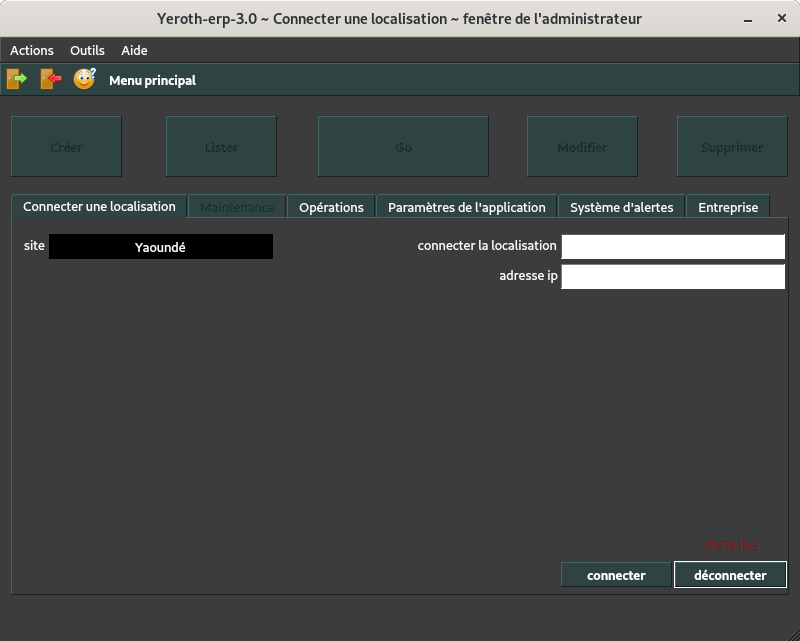
\includegraphics[scale=0.45]{images/yeroth-fenetre-administrateur.png}
\caption{La fen\^etre de l'administrateur.}
\label{fig:fenetre-administrateur}
\end{figure}

La figure~\ref{fig:fenetre-administrateur} illustre la
fen\^etre d'acceuil de l'administration de \yeren.

On y arrive automatiquement lorsqu'on s'enregistre
\`a \yeren avec un utilisateur du \role \admin.

Avec un utilisateur du \role \manager, on clique sur le
bouton \bouton{Administration} \`a partir de l'interface
d'acceuil des utilisateurs du \role \manager 
(voir figure~\ref{fig:yeren-fenetre-patron}).

\newpage

%%%%%%%%%%%%%%%%%%%%%%%%%%%%%%%%%%%%%%%%%%%%%%%%%%%%%%%%%%%%%%%%%%%%%%%%%%%%%%%%%

\nxsection{La connection \`a d'autres localisations}
\index{connection \`a d'autres localisations}

La figure~\ref{fig:yeren-admin-connection-autres-db}
illustre l'interface graphique de connection \`a la
base de donn\'ees d'une autre localisation;
cette interface graphique est le $1^{\text{er}}$ onglet
de la fen\^etre de l'administration.

\begin{figure}[!htpb]
	\centering
	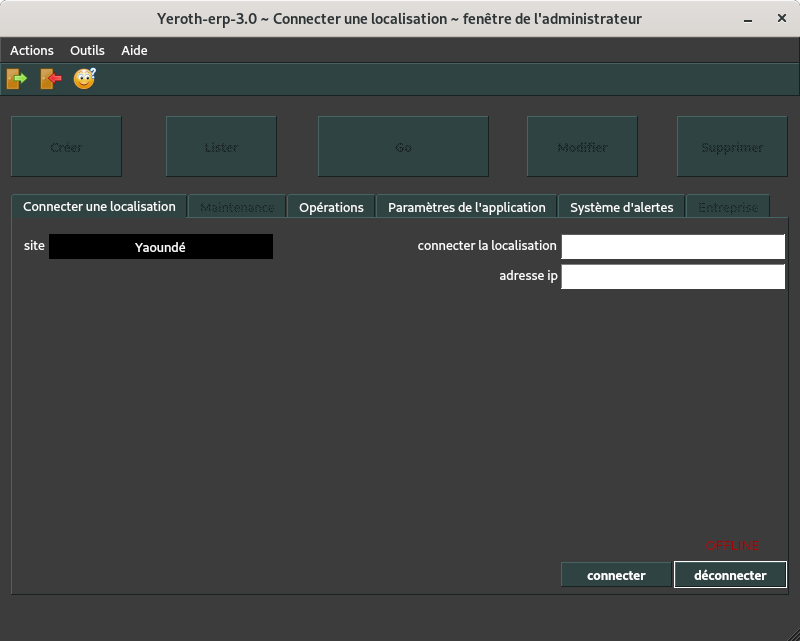
\includegraphics[scale=0.45]{images/yeren-admin-connection-autres-db.png}
	\caption{l'interface graphique de connection de
		\yeren \`a d'autres localisations.}\label{fig:yeren-admin-connection-autres-db}
\end{figure}

Voici la proc\'edure par laquelle l'utilisateur peut
connecter son installation de \yeren \`a la base de donn\'ees
d'autres localisations:
\begin{enumerate}[1)]
	\item choisir dans le champs de texte '\textbf{localisation}'
		le nom de localisation \`a laquelle on souhaite
		se connecter. Lorsque cela est fait, l'adresse IP
		de la localisation choisie est automatiquement
		affich\'ee dans le champs de texte '\textbf{adresse IP}'
	
	\item cliquer sur le bouton \bouton{connecter}.
\end{enumerate}

Si la connection est r\'eussie, le mot 
'\textbf{\textcolor{forestgreen}{ONLINE}}' est affich\'e en
couleur verte au dessus du bouton \bouton{connecter}.

%%%%%%%%%%%%%%%%%%%%%%%%%%%%%%%%%%%%%%%%%%%%%%%%%%%%%%%%%%%%%%%%%%%%%%%%%%%%%%%%%

\nxsection{Les param\`etres g\'en\'eraux}
\index{param\`etres g\'en\'eraux}

La figure~\ref{fig:yeren-parametres} illustre l'interface
graphique des param\`etres g\'en\'eraux de \yeren;
cette interface graphique est le $4^{\text{\`eme}}$
onglet de la fen\^etre de l'administration de \yeren.

\begin{figure}[!htpb]
	\centering
	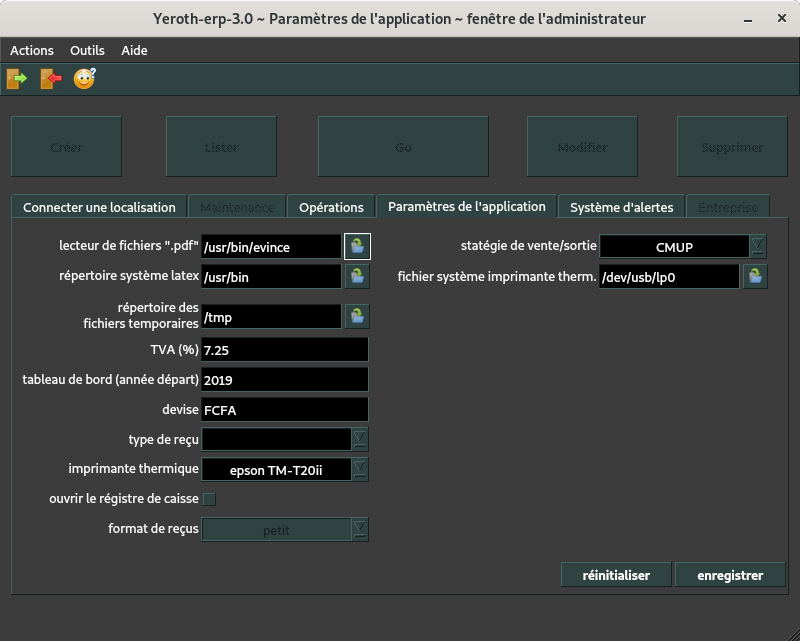
\includegraphics[scale=0.45]{images/yeroth-administration-parametres-generaux.png}
	\caption{l'interface graphique de param\'etrage g\'en\'eral
		de \yeren.}\label{fig:yeren-parametres}
\end{figure}

Les param\`etres g\'en\'eraux qui peuvent \^etre
modifi\'es sont les suivants:
\begin{enumerate}[1)]
	\item le lecteur des fichiers PDF
	\item le compilateur des fichiers '.tex'
	\item le r\'epertoire des fichiers temporaraires
	\item la taxe sur la valeur ajout\'e
	\item la strat\'egie de vente/sortie des stocks (\cmup, \dpfdpo, \fifo, \lifo)
		\begin{enumerate}[1)]
			\item la s\'election de \cmup pr\'esente tous les
				stocks pr\'esents dans la base de donn\'ees \index{\cmup}
			\item la s\'election \dpfdpo pr\'esente tous les
				stocks selon la strat\'egie ''\textbf{Date of Preemption,
				First Date of Preemption Out}'' \index{\dpfdpo}				
			\item la s\'election de \fifo pr\'esente tous les
				stocks selon la start\'egie ''\textbf{First In, First Out}''
				\index{\fifo}
			\item la s\'election de \lifo pr\'esente tous les
				stocks selon la strat\'egie ''\textbf{Last In, First Out}''
				\index{\lifo}
		\end{enumerate}
	\item le format des fichiers de facturations
	\item l'ann\'ee de d\'epart des rapports lors de la
			g\'en\'eration des chiffres d'affaire.\\
\end{enumerate}

Les strat\'egies de gestion des stocks sont d\'ecrites
dans la section~\ref{sec:strategies-gestion-stocks}.

%%%%%%%%%%%%%%%%%%%%%%%%%%%%%%%%%%%%%%%%%%%%%%%%%%%%%%%%%%%%%%%%%%%%%%%%%%%%%%%%%

\newpage
\nxsection{Les param\`etres du syst\`eme d'alertes}
\index{param\`etres du syst\`eme d'alertes}

La figure~\ref{fig:yeren-admin-alertes-config} illustre
l'interface graphique des param\`etres du syst\`eme d'alertes
de \yeren; cette interface graphique est le $5^{\text{\`eme}}$
onglet de la fene\^etre de l'administration de \yeren.

\begin{figure}[!htpb]
	\centering
	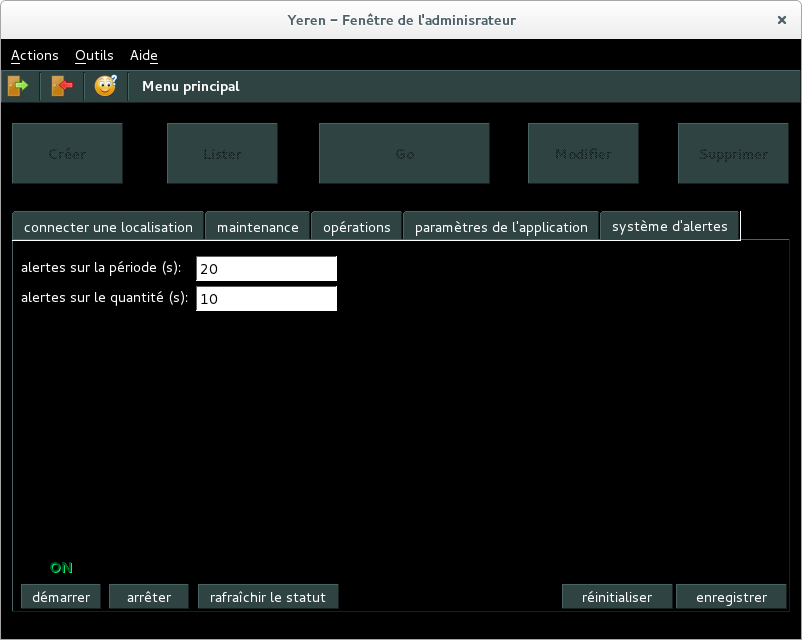
\includegraphics[scale=0.45]{images/yeren-admin-alertes-config.png}
	\caption{l'interface graphique de param\'etrage du
		syst\`eme d'alertes \yeren.}\label{fig:yeren-admin-alertes-config}
\end{figure}

Le syst\`eme d'alertes est d\'emarr\'e par d\'efaut lors du
d\'emarrage de l'ordinateur. 

Il faut d\'emarrer l'interface graphique de \yeren en tant
qu'administrateur du syst\`eme d'exploitation afin de
pouvoir stopper le syst\`eme d'alertes lorsqu'il a \'et\'e
d\'emarr\'e lors du d\'emarrage de l'ordinateur.

Les param\`etres du syst\`eme d'alertes qui peuvent \^etre
modifi\'es sont les suivants:
\begin{enumerate}[1)]
	\item \textbf{alertes sur la p\'eriode (s)}: d\'efinit
		l'intervalle de temps (en secondes) apr\`es lequel
		\yeren visite la base de donn\'ees pour voir
		s'il y'a de nouvelles alertes sur les p\'eriodes de temps
		
	\item \textbf{alertes sur la quantit\'e (s)}: d\'efinit
		l'intervalle de temps (en secondes) apr\`es lequel
		\yeren visite la base de donn\'ees pour voir
		s'il y'a de nouvelles alertes sur les quantit\'es en stocks.\\
\end{enumerate}

Cette interface graphique permet aussi:
\begin{enumerate}[1)]
	\item de \textbf{d\'emarrer le syst\`eme d'alertes} en pressant
		sur le bouton \bouton{d\'emarrer}. Lorsque le syst\`eme
		d'alertes est en marche, le mot anglais
		'\textbf{\textcolor{forestgreen}{ON}}' est
		affich\'e en vert au dessus du boutton \bouton{d\'emarrer}.
		
	\item \textbf{d'arr\^eter le syst\`eme d'alertes} en pressant
		sur le bouton \bouton{arr\^eter}. Lorsque le syst\`eme
		d'alertes n'est pas en marche, le mot anglais
		'\textbf{\textcolor{firebrickred}{OFF}}' est
		affich\'e en couleur rouge au dessus du boutton \bouton{arr\^eter}.
		
		Cette action n\'ecessite que l'utilisateur est d\'emarr\'e
		\yeren en tant qu'administrateur du syst\`eme d'exploitation.
		
	\item \textbf{d'actualiser le statut} dans lequel se trouve
		le syst\`eme d'alertes en pressant sur le bouton
		\bouton{rafra\^ichir le statut}.		
\end{enumerate}
%-----------------------------------------------------------

\newpage
\nxsection{Les Alertes}\label{sec:administration-alertes}
\index{les alertes}

\nxsubsection{Afficher les d\'etails d'une alerte}
\index{afficher les d\'etails d'une alerte}

La figure~\ref{fig:admin-alertes-afficher-details} illustre
l'interface graphique de \yeroth qui affiche les d\'etails
d'une alerte.\\

\begin{figure}[!htpb]
	\centering
	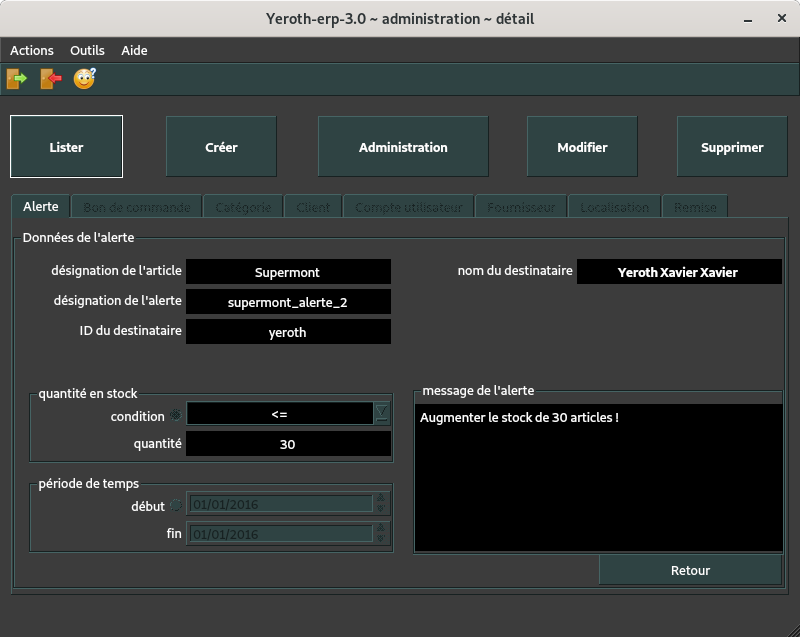
\includegraphics[scale=0.45]{images/alerte-afficher-details.png}
	\caption{Une interface graphique de \yeroth qui affiche les d\'etails
	d'une alerte.}\label{fig:admin-alertes-afficher-details}
\end{figure}

\procparagraph{Proc\'edure pour afficher les d\'etails d'une alerte}
\begin{enumerate}[1)]
	\item \`A partir de l'interface graphique de l'acceuil de
		l'administration (voir figure~\ref{fig:fenetre-administrateur}),
		on clique sur l'onglet intitul\'e \textbf{op\'erations}. 
		
	\item Choisir '\textbf{lister}' dans le '\emph{combo box
		op\'erations}'.
		
	\item Choisir '\textbf{une alerte}' dans le '\emph{combo box
		sujets}'. Vous \^etes automatiquement conduit \`a la fen\^etre
		illustr\'ee par la figure~\ref{fig:admin-alertes-lister}.
		
	\item S\'electionner l'alerte dont vous souhaitez afficher
		les d\'etails dans la liste des alertes affich\'ee.
		
	\item Cliquer sur le bouton \bouton{Afficher}. Les d\'etails
		sur le stock sont affich\'es dans une nouvelle fen\^etre.
\end{enumerate}

%%%%%%%%%%%%%%%%%%%%%%%%%%%%%%%%%%%%%%%%%%%%%%%%%%%%%%%%%%%%%%%%%%%%%%%%%%%%%%%%%

\newpage
\nxsubsection{Cr\'eer une alerte}\label{sec:administration-alertes-creer}
\index{cr\'eer une alerte}

La figure~\ref{fig:admin-alertes-creer} illustre l'interface
graphique de \yeroth pour cr\'eer une alerte.\\

\begin{figure}[!htpb]
	\centering
	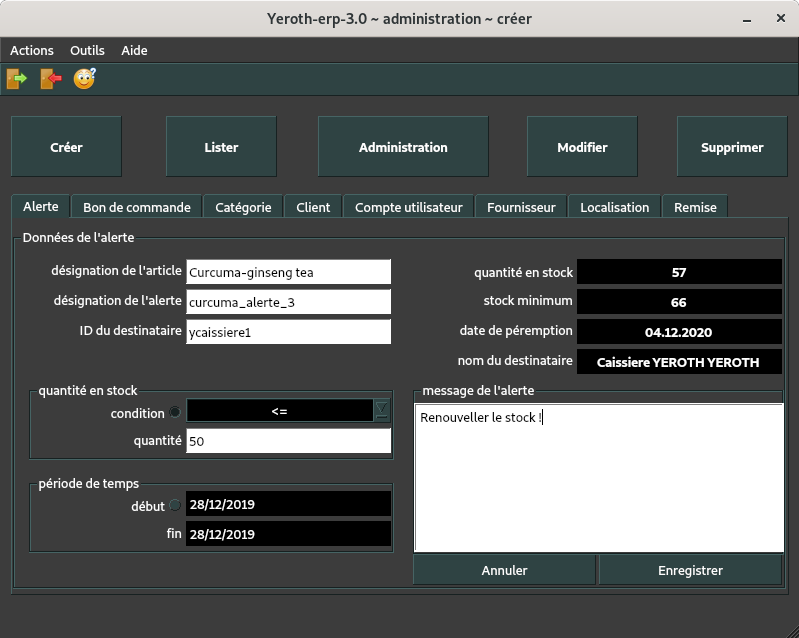
\includegraphics[scale=0.45]{images/alerte-creer.png}
	\caption{L'interface graphique pour cr\'eer des alertes.}
	\label{fig:admin-alertes-creer}
\end{figure}

\procparagraph{Proc\'edure pour cr\'eer une alerte}
Consulter les sections~\ref{sec:alerte-quantite-stock}
et~\ref{sec:alerte-periode-temps} pour savoir comment
cr\'eer respectivement des alertes sur la quantit\'e en
stock et des alertes sur la p\'eriode de temps.

%%%%%%%%%%%%%%%%%%%%%%%%%%%%%%%%%%%%%%%%%%%%%%%%%%%%%%%%%%%%%%%%%%%%%%%%%%%%%%%%%

\newpage
\nxsubsection{Lister les alertes}\label{sec:administration-alertes-lister}
\index{lister les alertes}

La figure~\ref{fig:admin-alertes-lister} illustre l'interface
graphique de \yeroth qui liste les alertes.\\

\begin{figure}[!htpb]
	\centering
	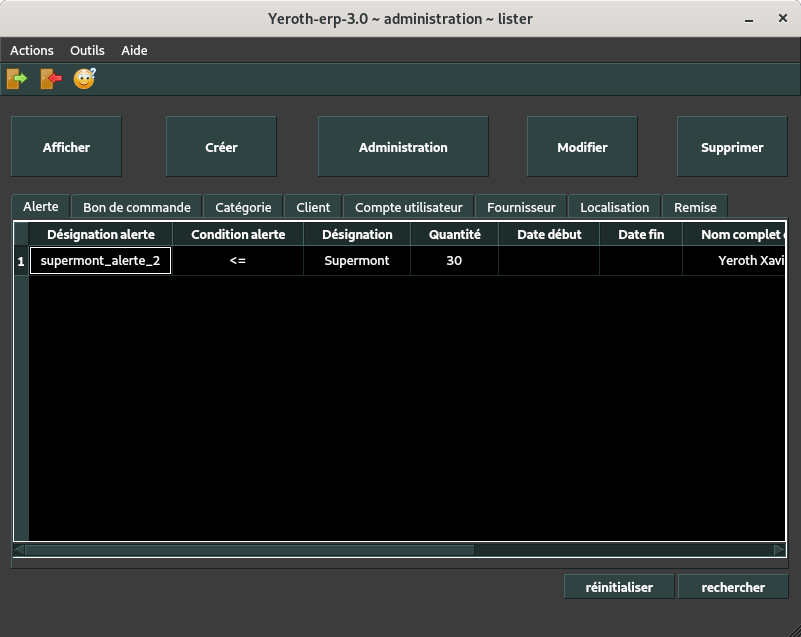
\includegraphics[scale=0.45]{images/alerte-lister.png}
	\caption{L'interface graphique qui liste les alertes.}
	\label{fig:admin-alertes-lister}
\end{figure}

\procparagraph{Proc\'edure pour lister les alertes}
\begin{enumerate}[1)]
	\item \`A partir de l'interface graphique de l'acceuil de
		l'administration (voir la figure~\ref{fig:fenetre-administrateur}),
		on clique sur l'onglet intitul\'e \textbf{op\'erations}. 
		
	\item Choisir '\textbf{lister}' dans le '\emph{combo box
		op\'erations}'.
		
	\item Choisir '\textbf{une alerte}' dans le '\emph{combo box
		sujets}'. Vous \^etes automatiquement conduit \`a la fen\^etre
		qui liste les alertes (voir la figure~\ref{fig:admin-alertes-lister}).
\end{enumerate}

%%%%%%%%%%%%%%%%%%%%%%%%%%%%%%%%%%%%%%%%%%%%%%%%%%%%%%%%%%%%%%%%%%%%%%%%%%%%%%%%%

\newpage
\nxsubsection{Modifier les d\'etails d'une alerte}
\index{modifier les d\'etails d'une alerte}

La figure~\ref{fig:admin-alertes-modifier} illustre
l'interface graphique de \yeroth pour modifier les
d\'etails d'une alerte.\\

\begin{figure}[!htpb]
	\centering
	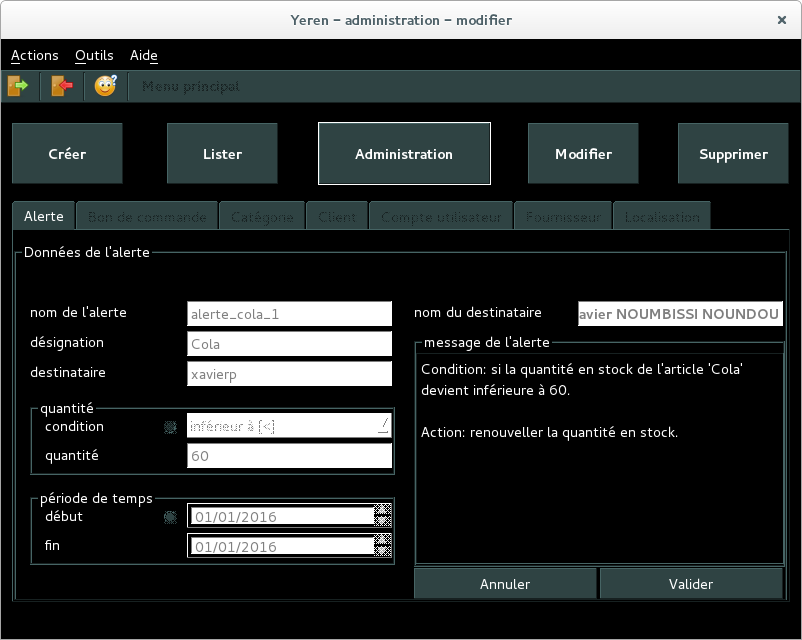
\includegraphics[scale=0.45]{images/alerte-modifier.png}
	\caption{L'interface graphique pour modifier les d'\'etails
	d'une alerte.}\label{fig:admin-alertes-modifier}
\end{figure}

\procparagraph{Proc\'edure pour modifier les d\'etails d'une alerte}
\begin{enumerate}[1)]
	\item \`A partir de l'interface graphique de l'acceuil de
		l'administration (voir figure~\ref{fig:fenetre-administrateur}),
		on clique sur l'onglet intitul\'e \textbf{op\'erations}. 
		
	\item Choisir '\textbf{lister}' dans le '\emph{combo box
		op\'erations}'.
		
	\item Choisir '\textbf{une alerte}' dans le '\emph{combo box
		sujets}'. Vous \^etes automatiquement conduit \`a la fen\^etre
		illustr\'ee par la figure~\ref{fig:admin-alertes-lister}.
		
	\item S\'electionner l'alerte dont vous souhaitez modifier
		les d\'etails dans la liste des alertes affich\'ee.
		
	\item Cliquer sur le bouton \bouton{Modifier}. Les d\'etails
		sur le stock sont affich\'es dans une nouvelle fen\^etre.
		
	\item Faites les modifications que vous souhaitez. Pour
		les alertes, seul le message d'alerte peut \^etre
		modifi\'e.
		
	\item Cliquer sur le bouton \bouton{valider} pour valider
		les modifications faites.
\end{enumerate}

%%%%%%%%%%%%%%%%%%%%%%%%%%%%%%%%%%%%%%%%%%%%%%%%%%%%%%%%%%%%%%%%%%%%%%%%%%%%%%%%%

\newpage
\nxsubsection{Supprimer une alerte}
\index{supprimer une alerte}

La figure~\ref{fig:admin-alertes-supprimer} illustre l'interface
graphique de \yeroth pour supprimer une alerte.\\

\begin{figure}[!htpb]
	\centering
	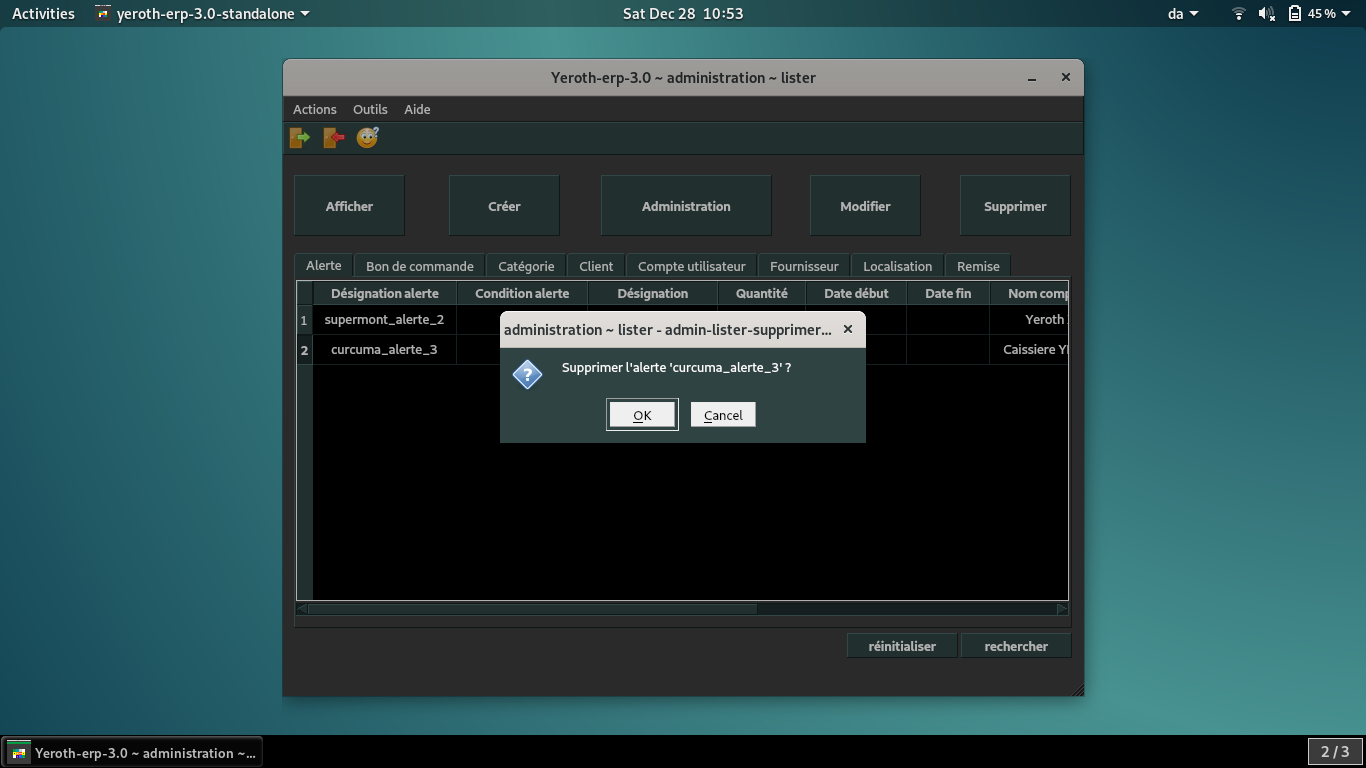
\includegraphics[scale=0.35]{images/alerte-supprimer.png}
	\caption{L'interface graphique pour supprimer des alertes.}
	\label{fig:admin-alertes-supprimer}
\end{figure}

\procparagraph{Proc\'edure pour supprimer une alerte}
\begin{enumerate}[1)]
	\item \`A partir de l'interface graphique de l'acceuil de
		l'administration (voir figure~\ref{fig:fenetre-administrateur}),
		on clique sur l'onglet intitul\'e \textbf{op\'erations}. 
		
	\item Choisir '\textbf{supprimer}' dans le '\emph{combo box
		op\'erations}'.
		
	\item Choisir '\textbf{une alerte}' dans le '\emph{combo box
		sujets}'. Vous \^etes automatiquement conduit \`a la fen\^etre
		illustr\'ee par la figure~\ref{fig:admin-alertes-lister}.
		
	\item S\'electionner l'alerte \`a supprimer dans la liste
		des alertes affich\'ee.
		
	\item Cliquer sur le bouton \bouton{Supprimer}. La question
		est ensuite pos\'ee si vous confirmer votre choix.
		Cliquer sur le \bouton{OK} pour confirmer votre choix.
\end{enumerate}

\newpage

%-----------------------------------------------------------

\nxsection{Les Cat\'egories d'Articles}
\index{les cat\'egories d'articles}

\nxsubsection{Afficher les d\'etails d'une cat\'egorie d'articles}
\index{afficher les d\'etails d'une cat\'egorie d'articles}
\index{d\'etails d'une cat\'egorie d'articles}

\begin{figure}[!htpb]
	\centering
	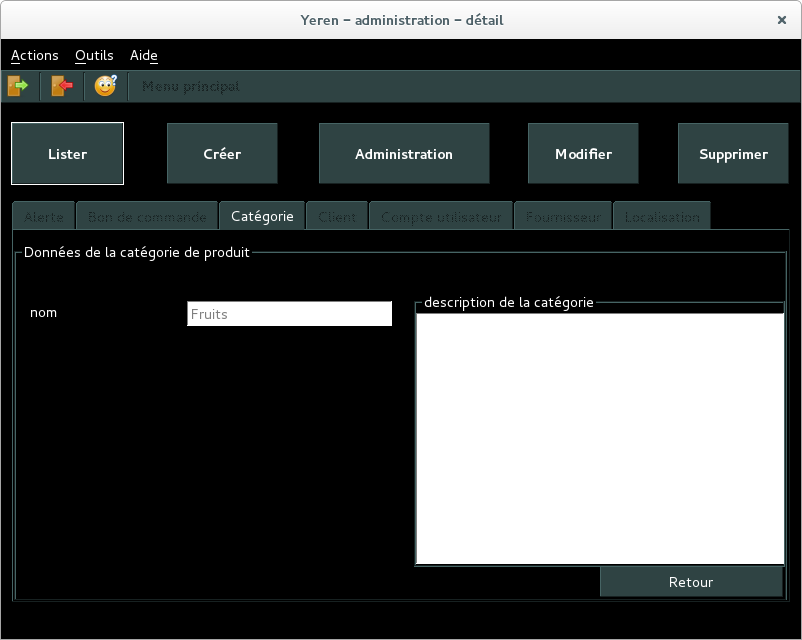
\includegraphics[scale=0.45]{images/categorie-articles-afficher-details.png}
	\caption{L'interface graphique pour afficher les d\'etails d'une
			cat\'egorie d'articles.}
	\label{fig:admin-categories-articles-afficher-details}
\end{figure}

La figure~\ref{fig:admin-categories-articles-afficher-details}
illustre l'interface graphique de \yeren qui affiche
les d\'etails d'une cat\'egorie d'articles.

\procparagraph{Proc\'edure pour afficher les d\'etails
	d'une cat\'egorie d'articles}
\begin{enumerate}[1)]
	\item \`A partir de l'interface graphique de l'acceuil de
		l'administration (voir figure~\ref{fig:fenetre-administrateur}),
		on clique sur l'onglet intitul\'e \textbf{op\'erations}. 
		
	\item Choisir '\textbf{lister}' dans le '\emph{combo box
		op\'erations}'.
		
	\item Choisir '\textbf{une cat\'egorie d'articles}' dans le
		'\emph{combo box objets}'. Vous \^etes automatiquement
		conduit \`a la fen\^etre illustr\'ee par la
		figure~\ref{fig:admin-categories-articles-lister}.
		
	\item S\'electionner la cat\'egorie d'articles dont vous
		souhaitez afficher les d\'etails.
		
	\item Cliquer sur le bouton \bouton{Afficher}. Les d\'etails
		sur la cat\'egorie d'articles sont affich\'es dans une
		nouvelle fen\^etre.
\end{enumerate}

%%%%%%%%%%%%%%%%%%%%%%%%%%%%%%%%%%%%%%%%%%%%%%%%%%%%%%%%%%%%%%%%%%%%%%%%%%%%%%%%%

\newpage
\nxsubsection{Cr\'eer une cat\'egorie d'articles}
\index{cr\'eer une cat\'egorie d'articles}

\begin{figure}[!htpb]
	\centering
	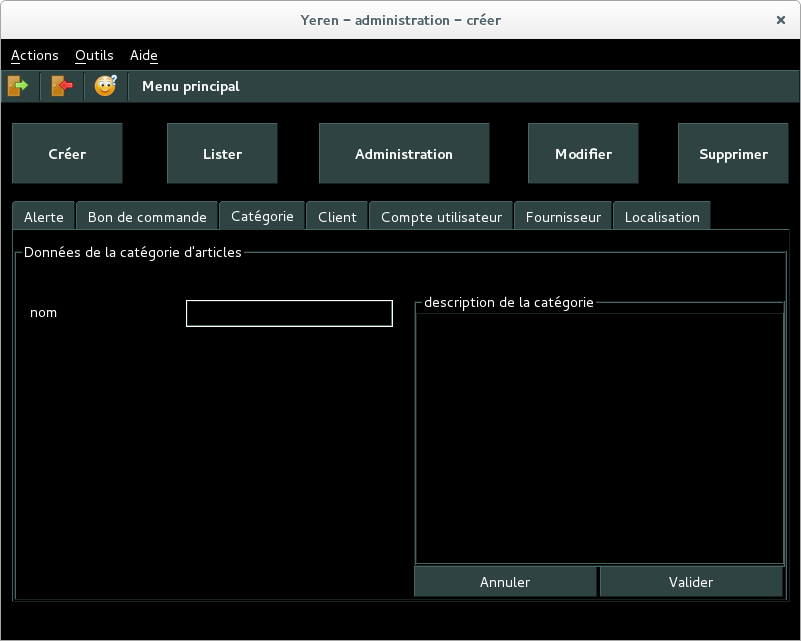
\includegraphics[scale=0.45]{images/categorie-articles-creer.png}
	\caption{L'interface graphique pour cr\'eer une cat\'egorie d'articles.}
	\label{fig:admin-categories-articles-creer}
\end{figure}

La figure~\ref{fig:admin-categories-articles-creer} illustre
l'interface graphique de \yeren pour cr\'eer une nouvelle
cat\'egorie d'articles.

\procparagraph{Proc\'edure pour cr\'eer une cat\'egorie d'articles}
\begin{enumerate}[1)]
	\item \`A partir de l'interface graphique de l'acceuil de
		l'administration (voir figure~\ref{fig:fenetre-administrateur}),
		on clique sur l'onglet intitul\'e \textbf{op\'erations}. 
		
	\item Choisir '\textbf{cr\'eer}' dans le '\emph{combo box
		op\'erations}'.
		
	\item Choisir '\textbf{une cat\'egorie d'articles}' dans
		le '\emph{combo box objets}'. Vous \^etes automatiquement
		conduit \`a la fen\^etre illustr\'ee par la
		figure~\ref{fig:admin-categories-articles-creer}.
		
	\item Saisissez la d\'esignation de la nouvelle cat\'egorie
		d'articles \`a cr\'eer dans le champs de texte
		'\textbf{d\'esignation}'.

	\item Si vous le souhaitez, saisisser un texte qui d\'ecrit
		cette nouvelle cat\'egorie d'articles dans le champs de
		texte '\textbf{description de la cat\'egorie}'.
		
	\item Cliquer sur le bouton \bouton{Valider} pour
		valider votre travail.		
\end{enumerate}

%%%%%%%%%%%%%%%%%%%%%%%%%%%%%%%%%%%%%%%%%%%%%%%%%%%%%%%%%%%%%%%%%%%%%%%%%%%%%%%%%

\newpage
\nxsubsection{Lister les cat\'egories d'articles}\label{sec:administration-categorie-lister}
\index{lister les cat\'egories d'articles}

\begin{figure}[!htpb]
	\centering
	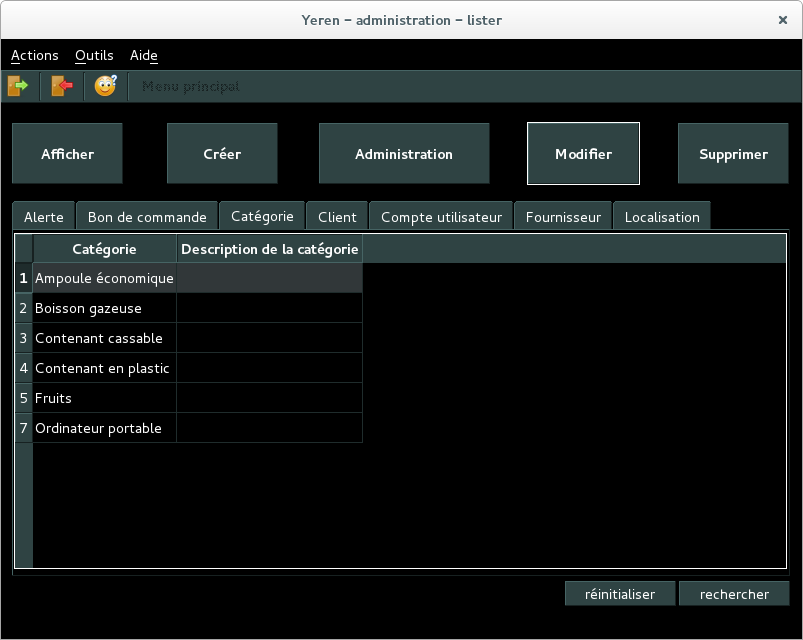
\includegraphics[scale=0.45]{images/categorie-articles-lister.png}
	\caption{L'interface graphique qui liste les cat\'egories d'articles.}
	\label{fig:admin-categories-articles-lister}
\end{figure}

La figure~\ref{fig:admin-categories-articles-lister} illustre
l'interface graphique de \yeren qui liste les cat\'egories
d'articles.

\procparagraph{Proc\'edure pour lister les cat\'egories d'articles}
\begin{enumerate}[1)]
	\item \`A partir de l'interface graphique de l'acceuil de
		l'administration (voir figure~\ref{fig:fenetre-administrateur}),
		on clique sur l'onglet intitul\'e \textbf{op\'erations}. 
		
	\item Choisir '\textbf{lister}' dans le '\emph{combo box
		op\'erations}'.
		
	\item Choisir '\textbf{une cat\'egorie d'articles}' dans
		le '\emph{combo box objets}'. Vous \^etes automatiquement
		conduit \`a la fen\^etre qui liste les cat\'egories
		d'articles (figure~\ref{fig:admin-categories-articles-lister}).
\end{enumerate}

%%%%%%%%%%%%%%%%%%%%%%%%%%%%%%%%%%%%%%%%%%%%%%%%%%%%%%%%%%%%%%%%%%%%%%%%%%%%%%%%%

\newpage
\nxsubsection{Modifier les d\'etails d'une cat\'egorie d'articles}
\index{modifier les d\'etails d'une cat\'egorie d'articles}

\begin{figure}[!htpb]
	\centering
	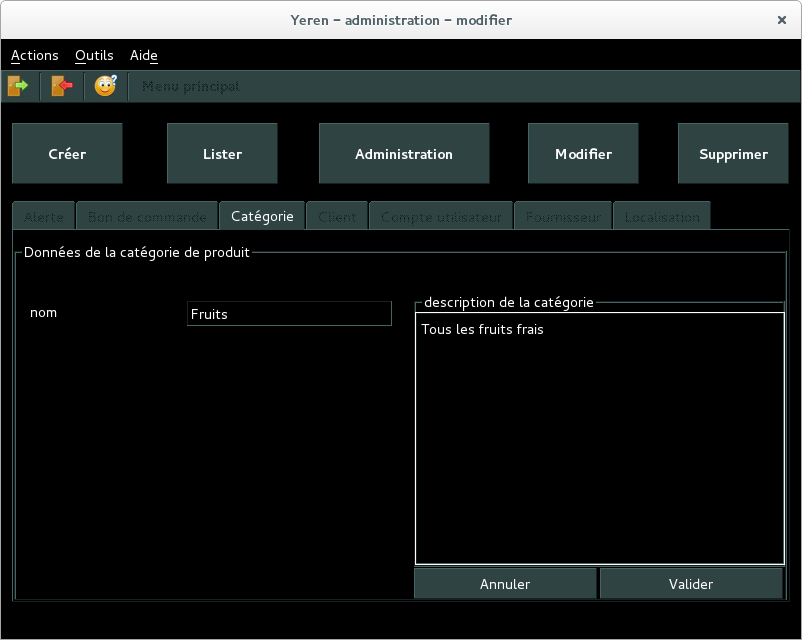
\includegraphics[scale=0.45]{images/categorie-articles-modifier.png}
	\caption{L'interface graphique pour modifier les d'\'etails
			d'une cat\'egorie d'articles.}
	\label{fig:admin-categories-articles-modifier}
\end{figure}

La figure~\ref{fig:admin-categories-articles-modifier}
illustre l'interface graphique de \yeren pour modifier
les d\'etails d'une cat\'egorie d'articles.

\procparagraph{Proc\'edure pour modifier les d\'etails
	d'une cat\'egorie d'articles}
\begin{enumerate}[1)]
	\item \`A partir de l'interface graphique de l'acceuil de
		l'administration (voir figure~\ref{fig:fenetre-administrateur}),
		on clique sur l'onglet intitul\'e \textbf{op\'erations}. 
		
	\item Choisir '\textbf{lister}' dans le '\emph{combo box
		op\'erations}'.
		
	\item Choisir '\textbf{cat\'egorie d'articles}' dans le
		'\emph{combo box objets}'. Vous \^etes automatiquement
		conduit \`a la fen\^etre illustr\'ee par la
		figure~\ref{fig:admin-categories-articles-lister}.
		
	\item S\'electionner l'alerte dont vous souhaitez modifier
		les d\'etails dans la liste	des d\'esignations des
		cat\'egories d'articles affich\'ee.
		
	\item Cliquer sur le bouton \bouton{Modifier}. Les d\'etails
		sur le stock sont affich\'es dans une nouvelle fen\^etre.
		
	\item Faites les modifications que vous souhaitez. Pour
		les alertes, seul le message d'alerte peut \^etre
		modifi\'e.
		
	\item Cliquer sur le bouton \bouton{valider} pour valider
		les modifications faites.
\end{enumerate}

%%%%%%%%%%%%%%%%%%%%%%%%%%%%%%%%%%%%%%%%%%%%%%%%%%%%%%%%%%%%%%%%%%%%%%%%%%%%%%%%%

\newpage
\nxsubsection{Supprimer une cat\'egorie d'article}
\index{supprimer une cat\'egorie d'article}

\begin{figure}[!htpb]
	\centering
	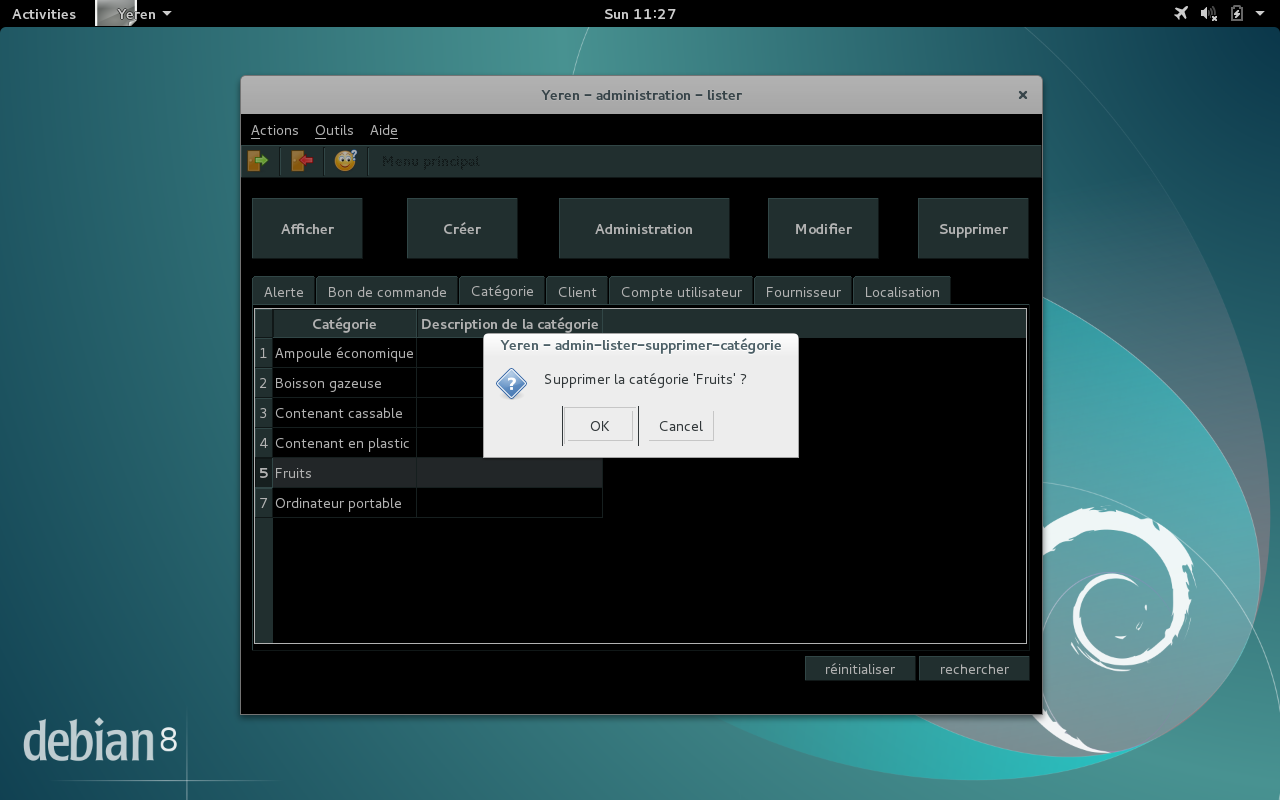
\includegraphics[scale=0.39]{images/categorie-articles-supprimer.png}
	\caption{L'interface graphique pour supprimer une cat\'egorie d'articles.}
	\label{fig:admin-categories-articles-supprimer}
\end{figure}

La figure~\ref{fig:admin-categories-articles-supprimer} illustre
l'interface graphique de \yeren pour supprimer une
cat\'egorie d'articles.

\procparagraph{Proc\'edure pour supprimer une cat\'egorie d'articles}
\begin{enumerate}[1)]
	\item \`A partir de l'interface graphique de l'acceuil de
		l'administration (voir figure~\ref{fig:fenetre-administrateur}),
		on clique sur l'onglet intitul\'e \textbf{op\'erations}. 
		
	\item Choisir '\textbf{supprimer}' dans le '\emph{combo box
		op\'erations}'.
		
	\item Choisir '\textbf{une cat\'egorie d'articles}' dans le
		'\emph{combo box objets}'. Vous \^etes automatiquement
		conduit \`a la fen\^etre illustr\'ee par la
		figure~\ref{fig:admin-categories-articles-lister}.
		
	\item S\'electionner l'alerte \`a supprimer dans la liste
		des d\'esignations des cat\'egories d'articles affich\'ee.
		
	\item Cliquer sur le bouton \bouton{Supprimer}. La question
		est ensuite pos\'ee si vous confirmer votre choix.
		Cliquer sur le \bouton{OK} pour confirmer votre choix.
\end{enumerate}

\newpage

%-----------------------------------------------------------

\nxsection{Les Comptes Clients}
\index{les comptes clients}

\nxsubsection{Afficher les d\'etails d'un compte client}
\index{afficher les d\'etails d'un compte client}

\begin{figure}[!htpb]
	\centering
	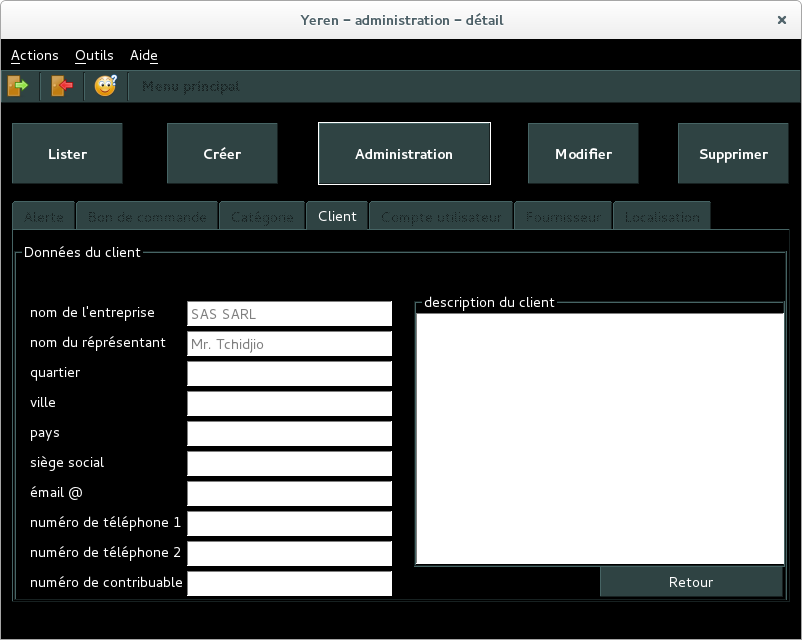
\includegraphics[scale=0.45]{images/compte-client-afficher-details.png}
	\caption{L'interface graphique pour afficher les d\'etails d'un compte client.}
	\label{fig:admin-compte-client-afficher-details}
\end{figure}

La figure~\ref{fig:admin-compte-client-afficher-details}
illustre l'interface graphique de \yeren qui affiche les
d\'etails d'un compte client.

\procparagraph{Proc\'edure pour afficher les d\'etails d'un compte client}
\begin{enumerate}[1)]
	\item \`A partir de l'interface graphique de l'acceuil de
		l'administration (voir figure~\ref{fig:fenetre-administrateur}),
		on clique sur l'onglet intitul\'e \textbf{op\'erations}. 
		
	\item Choisir '\textbf{lister}' dans le '\emph{combo box
		op\'erations}'.
		
	\item Choisir '\textbf{un compte client}' dans le '\emph{combo box
		sujets}'. Vous \^etes automatiquement conduit \`a la fen\^etre
		illustr\'ee par la figure~\ref{fig:admin-comptes-clients-lister}.
		
	\item S\'electionner le compte client dont vous souhaitez afficher
		les d\'etails dans la liste des comptes clients affich\'ee.
		
	\item Cliquer sur le bouton \bouton{Afficher}. Les d\'etails
		du compte client sont affich\'es dans une nouvelle fen\^etre.
\end{enumerate}

%------------------------------------------------------------------------------

\newpage
\nxsubsection{Cr\'eer un compte client}\label{sec:administration-comptes-clients-lister}
\index{cr\'eer un compte client}

\begin{figure}[!htpb]
	\centering
	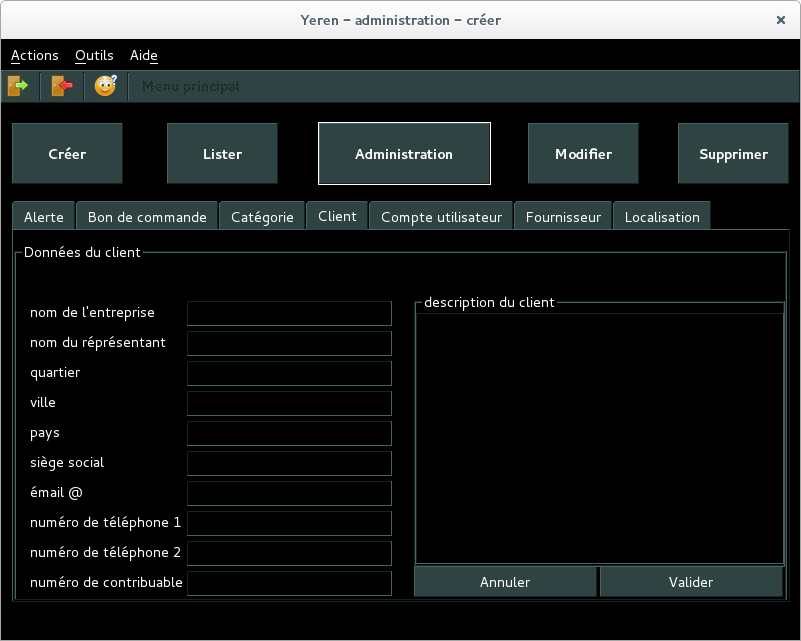
\includegraphics[scale=0.45]{images/compte-client-creer.png}
	\caption{L'interface graphique pour cr\'eer un compte client.}
	\label{fig:admin-comptes-clients-creer}
\end{figure}

La figure~\ref{fig:admin-comptes-clients-creer} illustre
l'interface graphique de \yeren pour cr\'eer un nouveau
compte client.

\procparagraph{Proc\'edure pour cr\'eer un compte client}
\begin{enumerate}[1)]
	\item \`A partir de l'interface graphique de l'acceuil de
		l'administration (voir figure~\ref{fig:fenetre-administrateur}),
		on clique sur l'onglet intitul\'e \textbf{op\'erations}. 
		
	\item Choisir '\textbf{cr\'eer}' dans le '\emph{combo box
		op\'erations}'.
		
	\item Choisir '\textbf{un compte client}' dans
		le '\emph{combo box objets}'. Vous \^etes automatiquement
		conduit \`a la fen\^etre illustr\'ee par la
		figure~\ref{fig:admin-comptes-clients-creer}.
		
	\item Saisissez les informations requises dans les champs de texte
		suivants:
		\begin{enumerate}[1)]
			\item nom de l'entreprise \obligatoire
			\item nom du r\'epr\'esentant \obligatoire
			\item quartier
			\item ville 
			\item pays
			\item si\`ege social 
			\item \'email@ 
			\item num\'ero de t\'el\'ephone 1 
			\item num\'ero de t\'el\'ephone 2
			\item num\'ero de contribuable 
			\item description du client.			
		\end{enumerate}
		
	\item Cliquer sur le bouton \bouton{Valider} pour
		valider votre travail.		
\end{enumerate}

%------------------------------------------------------------------------------

\newpage
\nxsubsection{Lister les comptes clients}\label{sec:administration-comptes-clients-lister}
\index{lister les comptes clients}

\begin{figure}[!htpb]
	\centering
	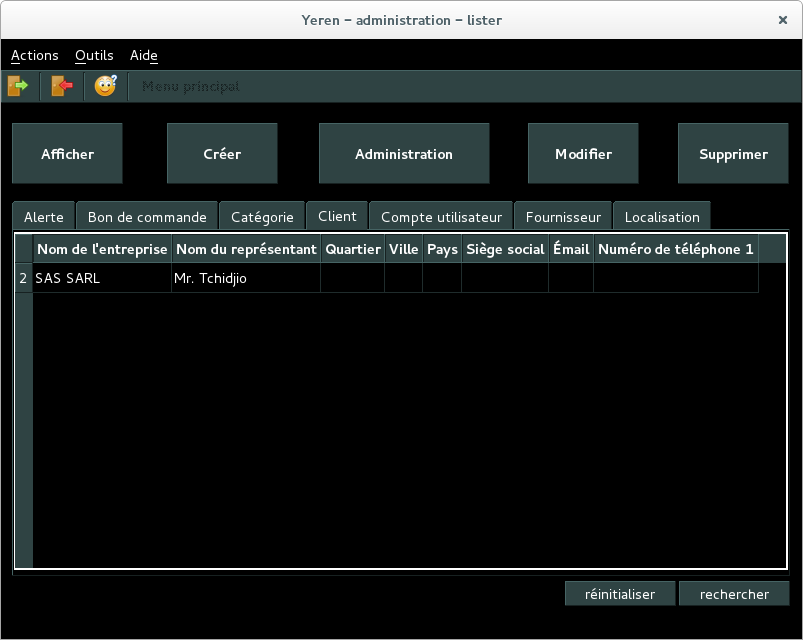
\includegraphics[scale=0.45]{images/compte-client-lister.png}
	\caption{L'interface graphique qui liste les comptes clients.}
	\label{fig:admin-comptes-clients-lister}
\end{figure}

La figure~\ref{fig:admin-comptes-clients-lister} illustre
l'interface graphique de \yeren qui liste les comptes clients.

\procparagraph{Proc\'edure pour lister les comptes clients}
\begin{enumerate}[1)]
	\item \`A partir de l'interface graphique de l'acceuil de
		l'administration (voir figure~\ref{fig:fenetre-administrateur}),
		on clique sur l'onglet intitul\'e \textbf{op\'erations}. 
		
	\item Choisir '\textbf{lister}' dans le '\emph{combo box
		op\'erations}'.
		
	\item Choisir '\textbf{un compte client}' dans
		le '\emph{combo box objets}'. Vous \^etes automatiquement
		conduit \`a la fen\^etre qui liste les comptes clients
		(figure~\ref{fig:admin-comptes-clients-lister}).
\end{enumerate}

%------------------------------------------------------------------------------

\newpage
\nxsubsection{Modifier les d\'etails d'un compte client}
\index{modifier les d\'etails d'un compte client}

\begin{figure}[!htpb]
	\centering
	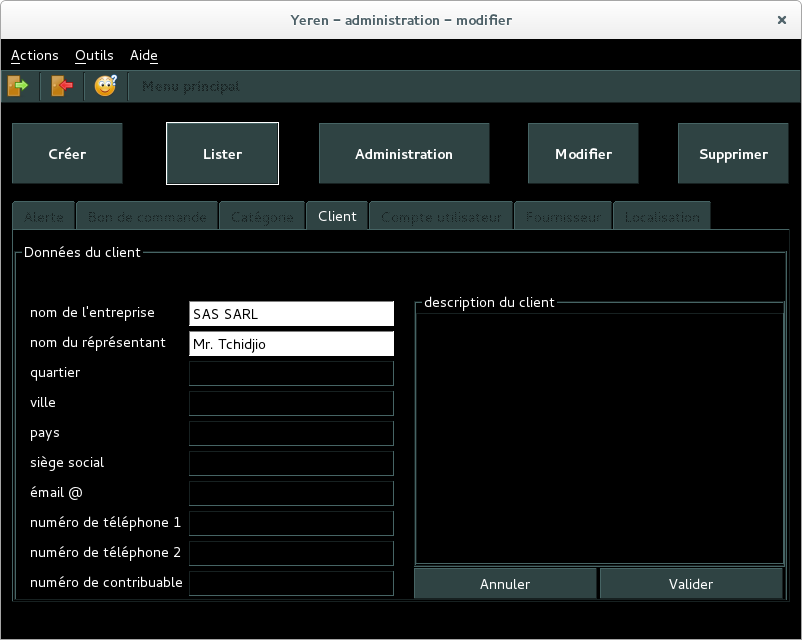
\includegraphics[scale=0.45]{images/compte-client-modifier.png}
	\caption{L'interface graphique pour modifier les d\'etails
			d'un compte client.}
	\label{fig:admin-comptes-clients-modifier}
\end{figure}

La figure~\ref{fig:admin-comptes-clients-modifier} illustre
l'interface graphique de \yeren pour modifier les
d\'etails d'un compte client.

\procparagraph{Proc\'edure pour modifier les d\'etails d'un compte client}
\begin{enumerate}[1)]
	\item \`A partir de l'interface graphique de l'acceuil de
		l'administration (voir figure~\ref{fig:fenetre-administrateur}),
		on clique sur l'onglet intitul\'e \textbf{op\'erations}. 
		
	\item Choisir '\textbf{lister}' dans le '\emph{combo box
		op\'erations}'.
		
	\item Choisir '\textbf{un compte client}' dans le '\emph{combo box
		sujets}'. Vous \^etes automatiquement conduit \`a la fen\^etre
		illustr\'ee par la figure~\ref{fig:admin-comptes-clients-lister}.
		
	\item S\'electionner le compte client dont vous souhaitez
		modifier les d\'etails dans la liste des comptes
		clients affich\'ee.
		
	\item Cliquer sur le bouton \bouton{Modifier}. Les d\'etails
		du compte client sont affich\'es dans une nouvelle fen\^etre.
		
	\item Faites les modifications que vous souhaitez.
		
	\item Cliquer sur le bouton \bouton{valider} pour valider
		les modifications faites.
\end{enumerate}

%------------------------------------------------------------------------------

\newpage
\nxsubsection{Supprimer un compte client}
\index{supprimer un compte client}

\begin{figure}[!htpb]
	\centering
	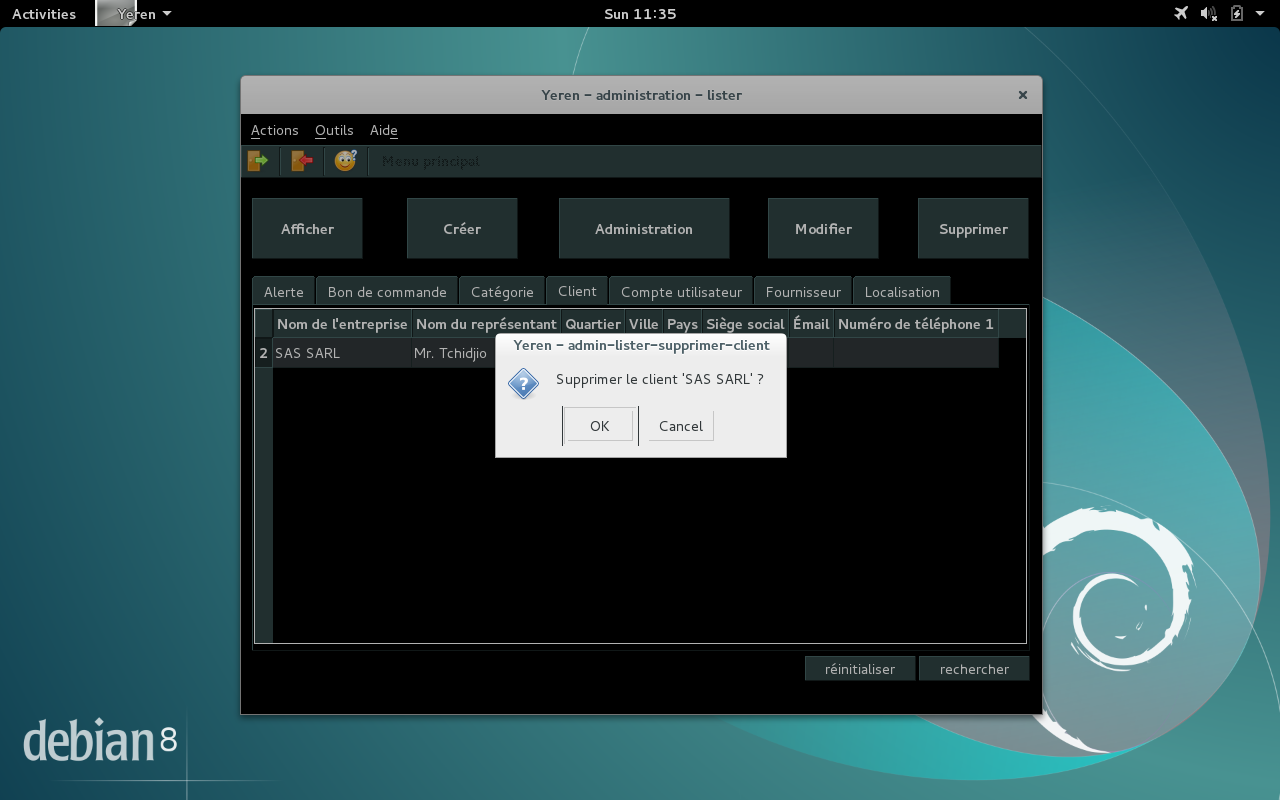
\includegraphics[scale=0.39]{images/compte-client-supprimer.png}
	\caption{L'interface graphique pour supprimer un compte client.}
	\label{fig:admin-comptes-clients-supprimer}
\end{figure}

La figure~\ref{fig:admin-comptes-clients-supprimer} illustre
l'interface graphique de \yeren pour supprimer un compte
client.

\procparagraph{Proc\'edure pour supprimer un compte client}
\begin{enumerate}[1)]
	\item \`A partir de l'interface graphique de l'acceuil de
		l'administration (voir figure~\ref{fig:fenetre-administrateur}),
		on clique sur l'onglet intitul\'e \textbf{op\'erations}. 
		
	\item Choisir '\textbf{supprimer}' dans le '\emph{combo box
		op\'erations}'.
		
	\item Choisir '\textbf{un compte client}' dans le '\emph{combo box
		sujets}'. Vous \^etes automatiquement conduit \`a la fen\^etre
		illustr\'ee par la figure~\ref{fig:admin-comptes-clients-lister}.
		
	\item S\'electionner le compte client \`a supprimer dans la liste
		des comptes clients affich\'ee.
		
	\item Cliquer sur le bouton \bouton{Supprimer}. La question
		est ensuite pos\'ee si vous confirmer votre choix.
		Cliquer sur le \bouton{OK} pour confirmer votre choix.
\end{enumerate}

\newpage

%-----------------------------------------------------------

\nxsection{Les Comptes Fournisseurs}
\index{les comptes fournisseurs}

\nxsubsection{Afficher les d\'etails d'un compte fournisseur}
\index{afficher les d\'etails d'un compte fournisseur}
\index{d\'etails d'un compte fournisseur}

\begin{figure}[!htpb]
	\centering
	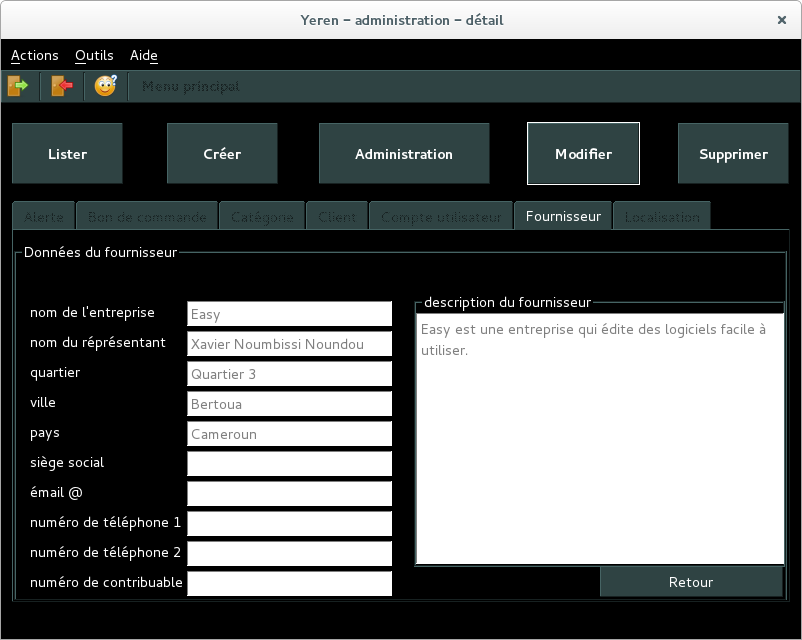
\includegraphics[scale=0.45]{images/compte-fournisseur-afficher-details.png}
	\caption{L'interface graphique pour afficher les d\'etails
			d'un compte fournisseur.}
	\label{fig:admin-fournisseurs-afficher-details}
\end{figure}

La figure~\ref{fig:admin-fournisseurs-afficher-details}
illustre l'interface graphique de \yeroth qui affiche
les d\'etails d'un compte fournisseur.

\procparagraph{Proc\'edure pour afficher les d\'etails
	d'un compte fournisseur}
\begin{enumerate}[1)]
	\item \`A partir de l'interface graphique de l'acceuil de
		l'administration (voir figure~\ref{fig:fenetre-administrateur}),
		on clique sur l'onglet intitul\'e \textbf{op\'erations}. 
		
	\item Choisir '\textbf{lister}' dans le '\emph{combo box
		op\'erations}'.
		
	\item Choisir '\textbf{un compte fournisseur}' dans le
		'\emph{combo box objets}'. Vous \^etes automatiquement
		conduit \`a la fen\^etre illustr\'ee par la
		figure~\ref{fig:admin-comptes-fournisseurs-lister}.
		
	\item S\'electionner le compte fournisseur dont vous
		souhaitez afficher les d\'etails dans la liste des
		comptes fournisseurs affich\'ee.
		
	\item Cliquer sur le bouton \bouton{Afficher}. Les d\'etails
		sur le compte fournisseur sont affich\'es dans une nouvelle.
\end{enumerate}

%%%%%%%%%%%%%%%%%%%%%%%%%%%%%%%%%%%%%%%%%%%%%%%%%%%%%%%%%%%%%%%%%%%%%%%%%%%%%%%%%

\newpage
\nxsubsection{Cr\'eer un compte fournisseur}
\index{cr\'eer un compte fournisseur}

\begin{figure}[!htpb]
	\centering
	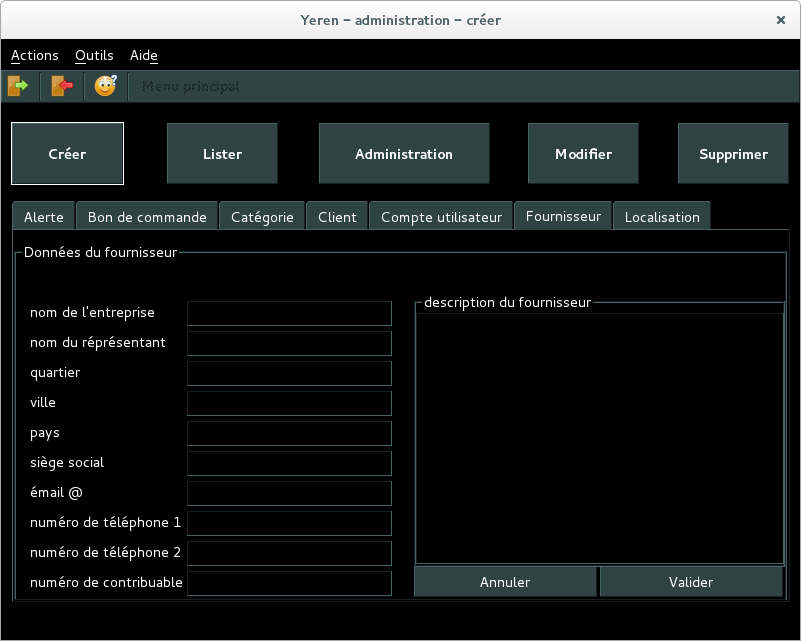
\includegraphics[scale=0.45]{images/compte-fournisseur-creer.png}
	\caption{L'interface graphique pour cr\'eer un
			nouveau compte fournisseur.}
	\label{fig:admin-comptes-fournisseurs-creer}
\end{figure}

La figure~\ref{fig:admin-comptes-fournisseurs-creer} illustre
l'interface graphique de \yeroth pour cr\'eer un nouveau
compte fournisseur.

\procparagraph{Proc\'edure pour cr\'eer un compte fournisseur}
\begin{enumerate}[1)]
	\item \`A partir de l'interface graphique de l'acceuil de
		l'administration (voir figure~\ref{fig:fenetre-administrateur}),
		on clique sur l'onglet intitul\'e \textbf{op\'erations}. 
		
	\item Choisir '\textbf{cr\'eer}' dans le '\emph{combo box
		op\'erations}'.
		
	\item Choisir '\textbf{un compte fournisseur}' dans
		le '\emph{combo box objets}'. Vous \^etes automatiquement
		conduit \`a la fen\^etre illustr\'ee par la
		figure~\ref{fig:admin-comptes-fournisseurs-creer}.
		
	\item Saisissez les informations requises dans les champs de texte
		suivants:
		\begin{enumerate}[1)]
			\item nom de l'entreprise \obligatoire
			\item nom du r\'epr\'esentant
			\item quartier
			\item ville 
			\item pays
			\item si\`ege social
			\item \'email@
			\item num\'ero de t\'el\'ephone 1
			\item num\'ero de t\'el\'ephone 2
			\item num\'ero de contribuable 
			\item description du fournisseur.
		\end{enumerate}
		
	\item Cliquer sur le bouton \bouton{Valider} pour
		valider votre travail.		
\end{enumerate}

%%%%%%%%%%%%%%%%%%%%%%%%%%%%%%%%%%%%%%%%%%%%%%%%%%%%%%%%%%%%%%%%%%%%%%%%%%%%%%%%%

\newpage
\nxsubsection{Lister les fournisseurs}
\index{lister les fournisseurs}

\begin{figure}[!htpb]
	\centering
	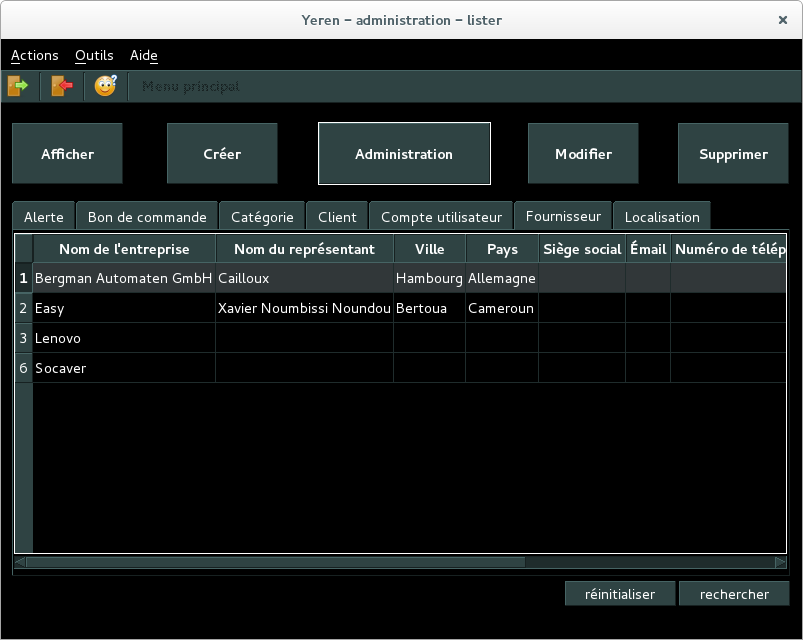
\includegraphics[scale=0.45]{images/compte-fournisseur-lister.png}
	\caption{L'interface graphique pour lister les comptes fournisseurs.}
	\label{fig:admin-comptes-fournisseurs-lister}
\end{figure}

La figure~\ref{fig:admin-comptes-fournisseurs-lister} illustre
l'interface graphique de \yeroth qui liste les comptes fournisseurs.

\procparagraph{Proc\'edure pour lister les comptes fournisseurs}
\begin{enumerate}[1)]
	\item \`A partir de l'interface graphique de l'acceuil de
		l'administration (voir figure~\ref{fig:fenetre-administrateur}),
		on clique sur l'onglet intitul\'e \textbf{op\'erations}. 
		
	\item Choisir '\textbf{lister}' dans le '\emph{combo box
		op\'erations}'.
		
	\item Choisir '\textbf{un compte fournisseur}' dans
		le '\emph{combo box objets}'. Vous \^etes automatiquement
		conduit \`a la fen\^etre qui liste les comptes fournisseurs
		(figure~\ref{fig:admin-comptes-fournisseurs-lister}).
\end{enumerate}

%%%%%%%%%%%%%%%%%%%%%%%%%%%%%%%%%%%%%%%%%%%%%%%%%%%%%%%%%%%%%%%%%%%%%%%%%%%%%%%%%

\newpage
\nxsubsection{Modifier les d\'etails d'un fournisseur}
\index{modifier les d\'etails d'un fournisseur}

\begin{figure}[!htpb]
	\centering
	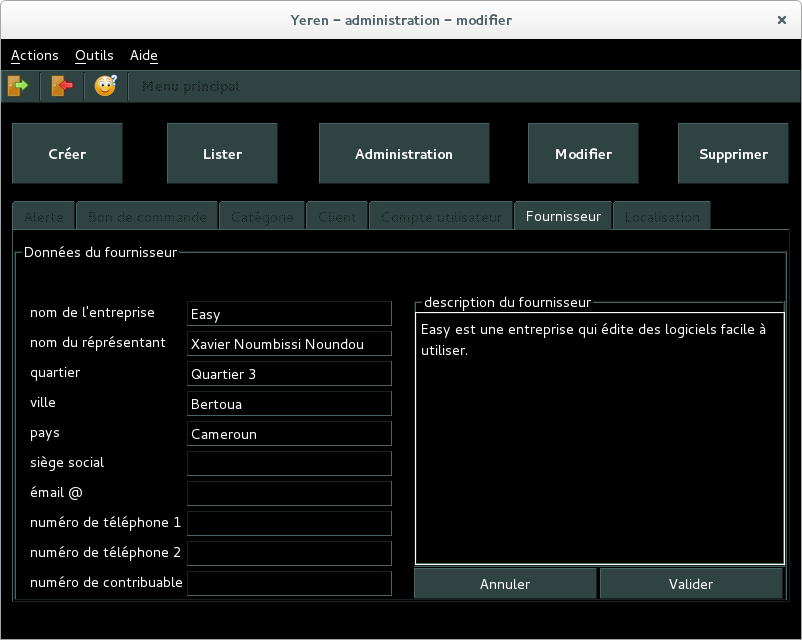
\includegraphics[scale=0.45]{images/compte-fournisseur-modifier.png}
	\caption{L'interface graphique pour modifier les
			d\'etails d'un compte fournisseur.}
	\label{fig:admin-comptes-fournisseurs-modifier}
\end{figure}

La figure~\ref{fig:admin-comptes-fournisseurs-modifier} illustre
l'interface graphique de \yeroth pour modifier les
d\'etails d'un compte fournisseur.

\procparagraph{Proc\'edure pour modifier les d\'etails d'un compte fournisseur}
\begin{enumerate}[1)]
	\item \`A partir de l'interface graphique de l'acceuil de
		l'administration (voir figure~\ref{fig:fenetre-administrateur}),
		on clique sur l'onglet intitul\'e \textbf{op\'erations}. 
		
	\item Choisir '\textbf{lister}' dans le '\emph{combo box
		op\'erations}'.
		
	\item Choisir '\textbf{un compte fournisseur}' dans le '\emph{combo box
		sujets}'. Vous \^etes automatiquement conduit \`a la fen\^etre
		illustr\'ee par la figure~\ref{fig:admin-comptes-fournisseurs-lister}.
		
	\item S\'electionner le compte fournisseur dont vous souhaitez
		modifier les d\'etails dans la liste des comptes fournisseurs
		affich\'ee.
		
	\item Cliquer sur le bouton \bouton{Modifier}. Les d\'etails
		du compte fournisseur sont affich\'es dans une nouvelle fen\^etre.
		
	\item Faites les modifications que vous souhaitez.
		
	\item Cliquer sur le bouton \bouton{valider} pour valider
		les modifications faites.
\end{enumerate}

%%%%%%%%%%%%%%%%%%%%%%%%%%%%%%%%%%%%%%%%%%%%%%%%%%%%%%%%%%%%%%%%%%%%%%%%%%%%%%%%%

\newpage
\nxsubsection{Supprimer un compte fournisseur}
\index{supprimer un compte fournisseur}

\begin{figure}[!htpb]
	\centering
	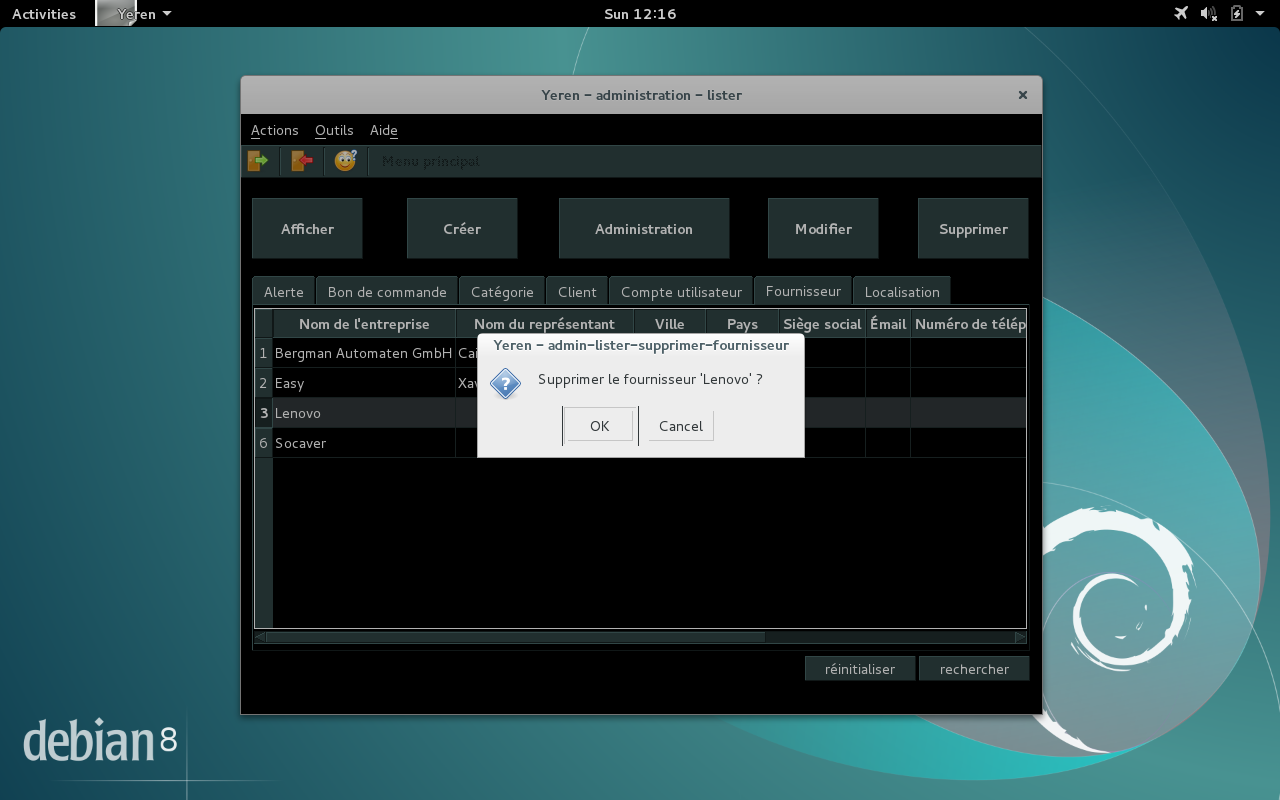
\includegraphics[scale=0.39]{images/compte-fournisseur-supprimer.png}
	\caption{L'interface graphique pour supprimer un fournisseur.}
	\label{fig:admin-comptes-fournisseurs-supprimer}
\end{figure}

La figure~\ref{fig:admin-comptes-fournisseurs-supprimer}
illustre l'interface graphique de \yeroth pour supprimer
un compte fournisseur.

\procparagraph{Proc\'edure pour supprimer un compte fournisseur}
\begin{enumerate}[1)]
	\item \`A partir de l'interface graphique de l'acceuil de
		l'administration (voir figure~\ref{fig:fenetre-administrateur}),
		on clique sur l'onglet intitul\'e \textbf{op\'erations}. 
		
	\item Choisir '\textbf{supprimer}' dans le '\emph{combo box
		op\'erations}'.
		
	\item Choisir '\textbf{un compte fournisseur}' dans le
		'\emph{combo box objets}'. Vous \^etes automatiquement
		conduit \`a la fen\^etre illustr\'ee par la
		figure~\ref{fig:admin-comptes-fournisseurs-lister}.
		
	\item S\'electionner le compte fournisseur \`a supprimer
		dans la liste des comptes fournisseurs affich\'ee.
		
	\item Cliquer sur le bouton \bouton{Supprimer}. La question
		est ensuite pos\'ee si vous confirmer votre choix.
		Cliquer sur le \bouton{OK} pour confirmer votre choix.
\end{enumerate}

\newpage

%-----------------------------------------------------------

\nxsection{Les Comptes Utilisateurs}
\index{les comptes utilisateurs}

\nxsubsection{Afficher les d\'etails d'un compte utilisateur}
\index{afficher les d\'etails d'un compte utilisateur}
\index{d\'etails d'un compte utilisateur}

\begin{figure}[!htpb]
	\centering
	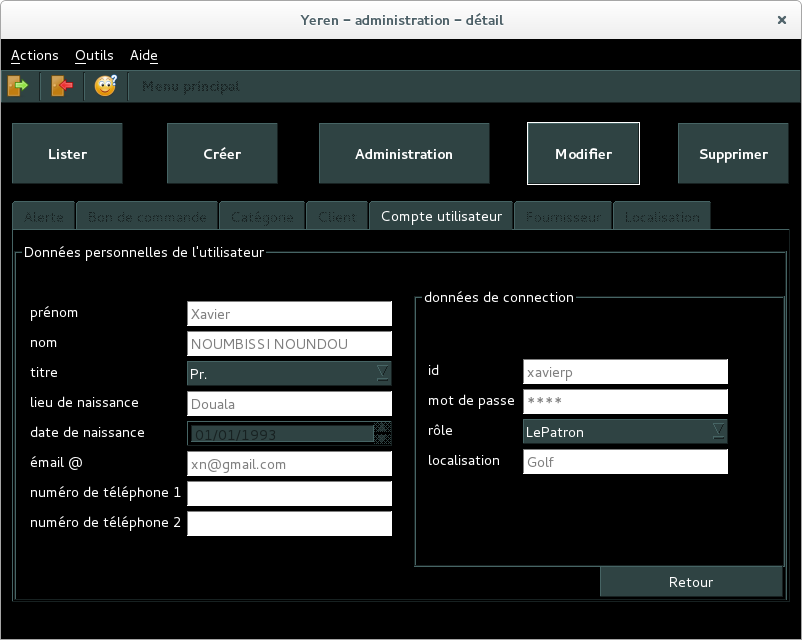
\includegraphics[scale=0.45]{images/compte-utilisateur-afficher-details.png}
	\caption{L'interface graphique pour afficher les d\'etails
			d'un compte utilisateur.}
	\label{fig:admin-comptes-utilisateurs-afficher-details}
\end{figure}

La figure~\ref{fig:admin-comptes-utilisateurs-afficher-details}
illustre l'interface graphique de \yeroth qui affiche les
d\'etails d'un compte utilisateur.

\procparagraph{Proc\'edure pour afficher les d\'etails d'un compte utilisateur}
\begin{enumerate}[1)]
	\item \`A partir de l'interface graphique de l'acceuil de
		l'administration (voir figure~\ref{fig:fenetre-administrateur}),
		on clique sur l'onglet intitul\'e \textbf{op\'erations}. 
		
	\item Choisir '\textbf{lister}' dans le '\emph{combo box
		op\'erations}'.
		
	\item Choisir '\textbf{un compte utilisateur}' dans le
		'\emph{combo box objets}'. Vous \^etes automatiquement
		conduit \`a la fen\^etre illustr\'ee par la
		figure~\ref{fig:admin-comptes-utilisateurs-lister}.
		
	\item S\'electionner le compte utilisateur dont vous
		souhaitez afficher les d\'etails dans la liste des
		comptes utilisateurs affich\'ee.
		
	\item Cliquer sur le bouton \bouton{Afficher}. Les d\'etails
		sur le compte utilisateur sont affich\'es dans
		une nouvelle fen\^etre.
\end{enumerate}

%%%%%%%%%%%%%%%%%%%%%%%%%%%%%%%%%%%%%%%%%%%%%%%%%%%%%%%%%%%%%%%%%%%%%%%%%%%%%%%%%

\newpage
\nxsubsection{Cr\'eer un compte utilisateur}
\index{cr\'eer un compte utilisateur}

\begin{figure}[!htpb]
	\centering
	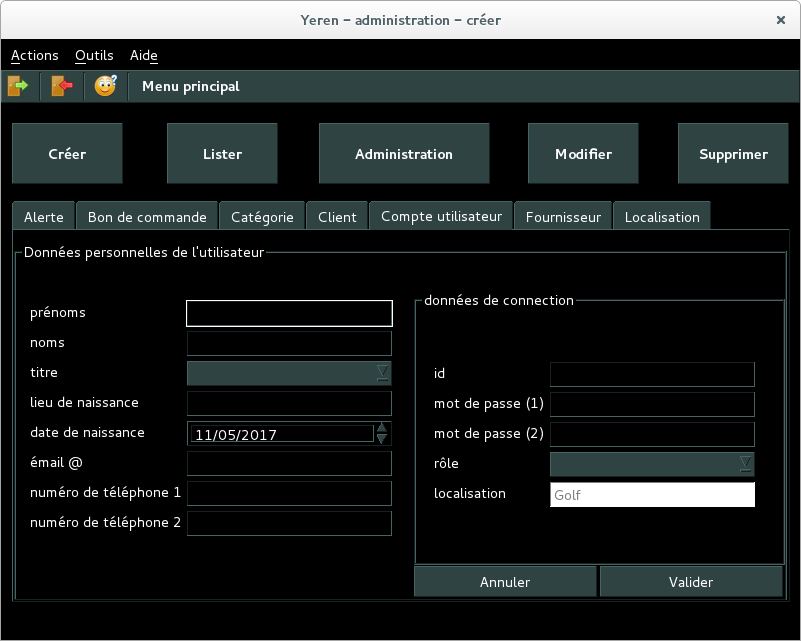
\includegraphics[scale=0.45]{images/compte-utilisateur-creer.png}
	\caption{L'interface graphique pour cr\'eer un compte utilisateur.}
	\label{fig:admin-comptes-utilisateurs-creer}
\end{figure}

La figure~\ref{fig:admin-comptes-utilisateurs-creer} illustre
l'interface graphique de \yeroth pour cr\'eer un nouveau
compte utilisateur.

\procparagraph{Proc\'edure pour cr\'eer un compte utilisateur}
\begin{enumerate}[1)]
	\item \`A partir de l'interface graphique de l'acceuil de
		l'administration (voir figure~\ref{fig:fenetre-administrateur}),
		on clique sur l'onglet intitul\'e \textbf{op\'erations}. 
		
	\item Choisir '\textbf{cr\'eer}' dans le '\emph{combo box
		op\'erations}'.
		
	\item Choisir '\textbf{un compte utilisateur}' dans
		le '\emph{combo box objets}'. Vous \^etes automatiquement
		conduit \`a la fen\^etre illustr\'ee par la
		figure~\ref{fig:admin-comptes-utilisateurs-creer}.
		
	\item Saisissez les informations requises dans les champs
		de texte suivants:
		\begin{enumerate}[1)]
			\item pr\'enoms \obligatoire
			\item noms \obligatoire
			\item titre	\obligatoire
			\item lieu de naissance 
			\item date de naissance
			\item ville
			\item province / \'etat
			\item pays
			\item bo\^ite postale
			\item \'email 
			\item num\'ero de t\'el\'ephone 1 
			\item num\'ero de t\'el\'ephone 2 
			\item nom d'utilisateur \obligatoire
			\item mot de passe \obligatoire
			\item v\'erification du mot de passe \obligatoire			
			\item r\^ole \obligatoire.
		\end{enumerate}
		
	\item Cliquer sur le bouton \bouton{Valider} pour
		valider votre travail.	
\end{enumerate}


%%%%%%%%%%%%%%%%%%%%%%%%%%%%%%%%%%%%%%%%%%%%%%%%%%%%%%%%%%%%%%%%%%%%%%%%%%%%%%%%%

\newpage
\nxsubsection{Lister les comptes utilisateurs}
\index{lister les comptes utilisateur}

\begin{figure}[!htpb]
	\centering
	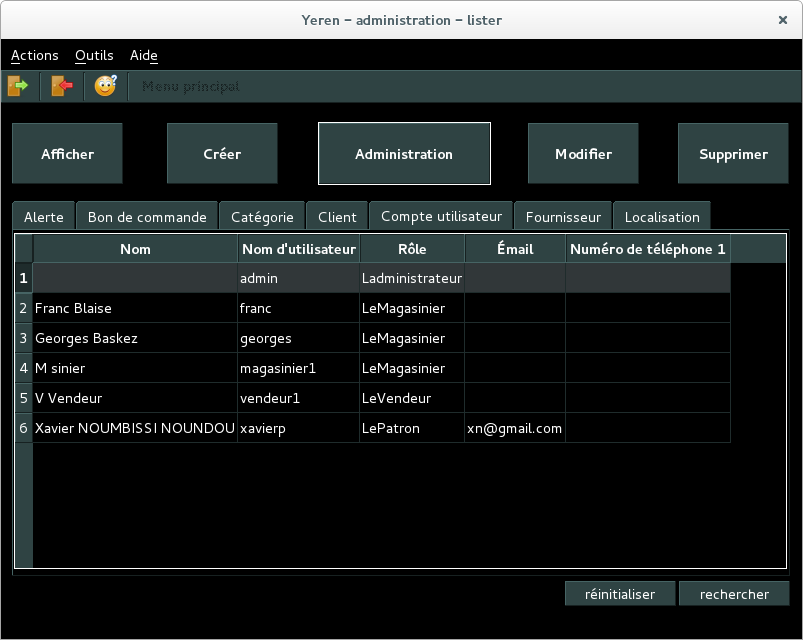
\includegraphics[scale=0.45]{images/compte-utilisateur-lister.png}
	\caption{L'interface graphique pour lister les comptes utilisateurs.}
	\label{fig:admin-comptes-utilisateurs-lister}
\end{figure}

La figure~\ref{fig:admin-comptes-utilisateurs-lister}
illustre l'interface graphique de \yeroth qui liste les
comptes utilisateurs.

\procparagraph{Proc\'edure pour lister les comptes utilisateurs}
\begin{enumerate}[1)]
	\item \`A partir de l'interface graphique de l'acceuil de
		l'administration (voir figure~\ref{fig:fenetre-administrateur}),
		on clique sur l'onglet intitul\'e \textbf{op\'erations}. 
		
	\item Choisir '\textbf{lister}' dans le '\emph{combo box
		op\'erations}'.
		
	\item Choisir '\textbf{un compte utilisateur}' dans
		le '\emph{combo box objets}'. Vous \^etes automatiquement
		conduit \`a la fen\^etre qui liste les comptes clients
		(figure~\ref{fig:admin-comptes-utilisateurs-lister}).
\end{enumerate}

%%%%%%%%%%%%%%%%%%%%%%%%%%%%%%%%%%%%%%%%%%%%%%%%%%%%%%%%%%%%%%%%%%%%%%%%%%%%%%%%%

\newpage
\nxsubsection{Modifier les d\'etails d'un compte utilisateur}
\index{modifier les d\'etails d'un compte utilisateur}

\begin{figure}[!htpb]
	\centering
	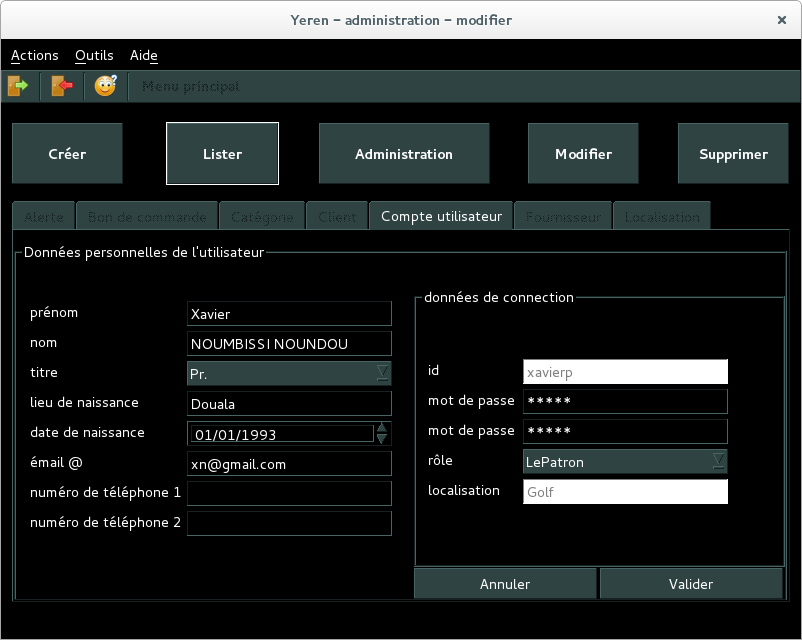
\includegraphics[scale=0.45]{images/compte-utilisateur-modifier.png}
	\caption{L'interface graphique pour modifier les d\'etails
			d'un compte utilisateur.}
	\label{fig:admin-comptes-utilisateurs-modifier}
\end{figure}

La figure~\ref{fig:admin-comptes-utilisateurs-modifier} illustre
l'interface graphique de \yeroth pour modifier les d\'etails
d'un compte utilisateur.

\procparagraph{Proc\'edure pour modifier les d\'etails d'un compte utilisateur}
\begin{enumerate}[1)]
	\item \`A partir de l'interface graphique de l'acceuil de
		l'administration (voir figure~\ref{fig:fenetre-administrateur}),
		on clique sur l'onglet intitul\'e \textbf{op\'erations}. 
		
	\item Choisir '\textbf{lister}' dans le '\emph{combo box
		op\'erations}'.
		
	\item Choisir '\textbf{un compte utilisateur}' dans
		le '\emph{combo box objets}'. Vous \^etes automatiquement
		conduit \`a la fen\^etre illustr\'ee par la
		figure~\ref{fig:admin-comptes-utilisateurs-lister}.
		
	\item S\'electionner le compte utilisateur dont vous souhaitez
		modifier les d\'etails dans la liste des comptes
		utilisateurs affich\'ee.
		
	\item Cliquer sur le bouton \bouton{Modifier}. Les d\'etails
		du compte utilisateur sont affich\'es dans une nouvelle fen\^etre.
		
	\item Faites les modifications que vous souhaitez.
		
	\item Cliquer sur le bouton \bouton{valider} pour valider
		les modifications faites.
\end{enumerate}

%%%%%%%%%%%%%%%%%%%%%%%%%%%%%%%%%%%%%%%%%%%%%%%%%%%%%%%%%%%%%%%%%%%%%%%%%%%%%%%%%

\newpage
\nxsubsection{Supprimer un compte utilisateur}
\index{supprimer un compte utilisateur}

\begin{figure}[!htpb]
	\centering
	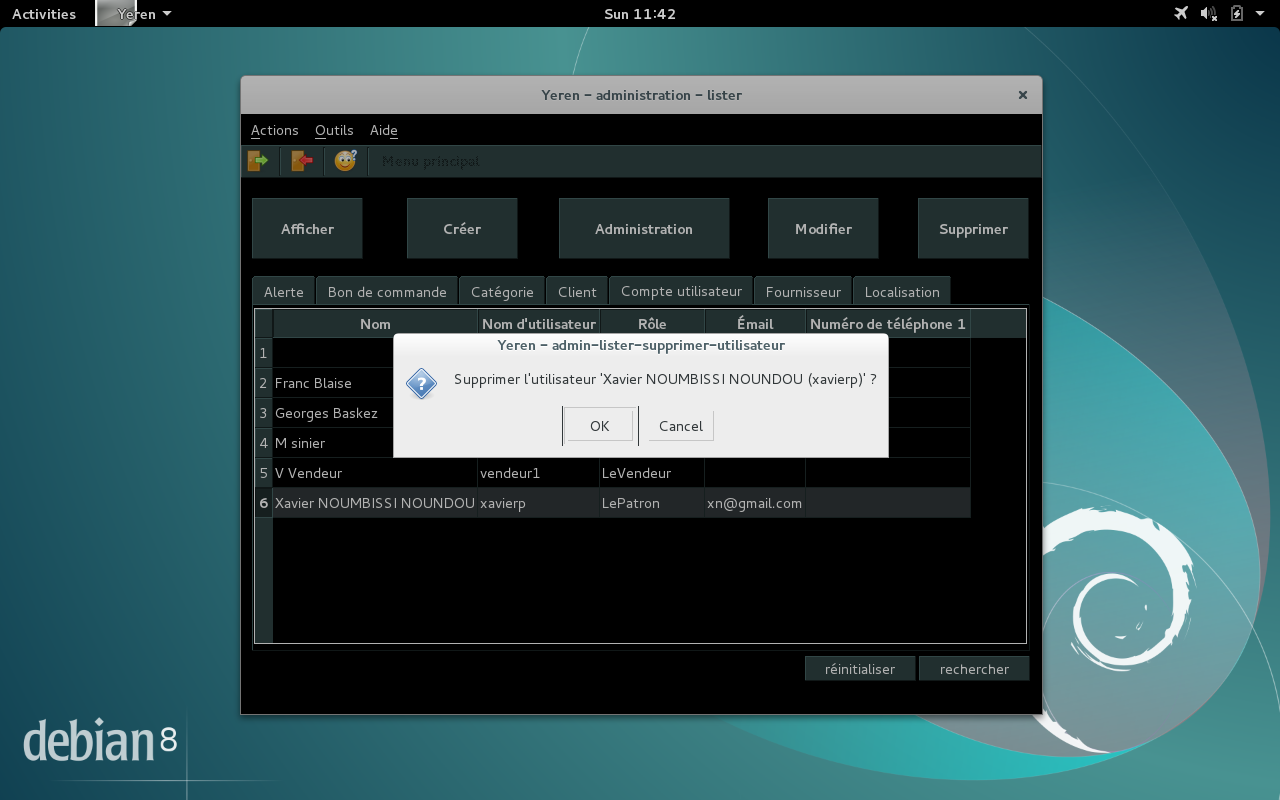
\includegraphics[scale=0.39]{images/compte-utilisateur-supprimer.png}
	\caption{L'interface graphique pour supprimer un compte utilisateur.}
	\label{fig:admin-comptes-utilisateurs-supprimer}
\end{figure}

La figure~\ref{fig:admin-comptes-utilisateurs-supprimer}
illustre l'interface graphique de \yeroth pour supprimer
un compte utilisateur.

\procparagraph{Proc\'edure pour supprimer un compte utilisateur}
\begin{enumerate}[1)]
	\item \`A partir de l'interface graphique de l'acceuil de
		l'administration (voir figure~\ref{fig:fenetre-administrateur}),
		on clique sur l'onglet intitul\'e \textbf{op\'erations}. 
		
	\item Choisir '\textbf{supprimer}' dans le '\emph{combo box
		op\'erations}'.
		
	\item Choisir '\textbf{un compte utilisateur}' dans le
		'\emph{combo box objets}'. Vous \^etes automatiquement
		conduit \`a la fen\^etre illustr\'ee par la
		figure~\ref{fig:admin-comptes-utilisateurs-lister}.
		
	\item S\'electionner le compte utilisateur \`a supprimer
		dans la liste des comptes utilisateurs affich\'ee.
		
	\item Cliquer sur le bouton \bouton{Supprimer}. La question
		est ensuite pos\'ee si vous confirmer votre choix.
		Cliquer sur le \bouton{OK} pour confirmer votre choix.
\end{enumerate}

\newpage

%-----------------------------------------------------------

\nxsection{Les Localisations}
\index{localisation}

Une localisation repr\'esente une boutique ou un d\'ep\^ot
de l'entreprise utilisant \yeren.

Les informations sur une localisation permettent de
se connecter \`a la base de donn\'ees de la boutique
ou du d\'ep\^ot qu'elle repr\'esente.

\nxsubsection{Afficher les d\'etails d'une localisation}
\index{afficher les d\'etails d'une localisation}
\index{d\'etails d'une localisation}

La figure~\ref{fig:admin-localisations-afficher-details} illustre
l'interface graphique de \yeren qui affiche les d\'etails
d'une localisation.\\

\begin{figure}[!htpb]
	\centering
	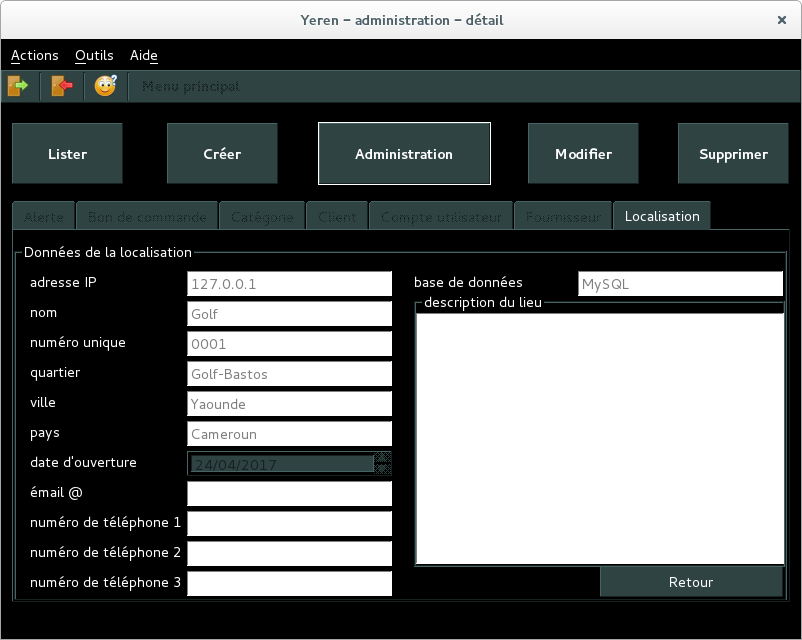
\includegraphics[scale=0.45]{images/localisation-afficher-details.png}
	\caption{L'interface graphique pour afficher les d\'etails
			d'une localisation.}
	\label{fig:admin-localisations-afficher-details}
\end{figure}

\procparagraph{Proc\'edure pour afficher les d\'etails d'une localisation}
\begin{enumerate}[1)]
	\item \`A partir de l'interface graphique de l'acceuil de
		l'administration (voir figure~\ref{fig:fenetre-administrateur}),
		on clique sur l'onglet intitul\'e \textbf{op\'erations}. 
		
	\item Choisir '\textbf{lister}' dans le '\emph{combo box
		op\'erations}'.
		
	\item Choisir '\textbf{une localisation}' dans le '\emph{combo box
		sujets}'. Vous \^etes automatiquement conduit \`a la fen\^etre
		illustr\'ee par la figure~\ref{fig:admin-localisations-lister}.
		
	\item S\'electionner la localisation dont vous souhaitez afficher
		les d\'etails dans la liste des localisations affich\'ee.
		
	\item Cliquer sur le bouton \bouton{Afficher}. Les d\'etails
		sur la localisation choisie sont affich\'es dans
		une nouvelle fen\^etre.
\end{enumerate}

%%%%%%%%%%%%%%%%%%%%%%%%%%%%%%%%%%%%%%%%%%%%%%%%%%%%%%%%%%%%%%%%%%%%%%%%%%%%%%%%%

\nxsubsection{Cr\'eer une localisation}
\index{cr\'eer une localisation}

La figure~\ref{fig:admin-localisations-creer} illustre
l'interface graphique de \yeren pour cr\'eer une localisation.\\

\begin{figure}[!htpb]
	\centering
	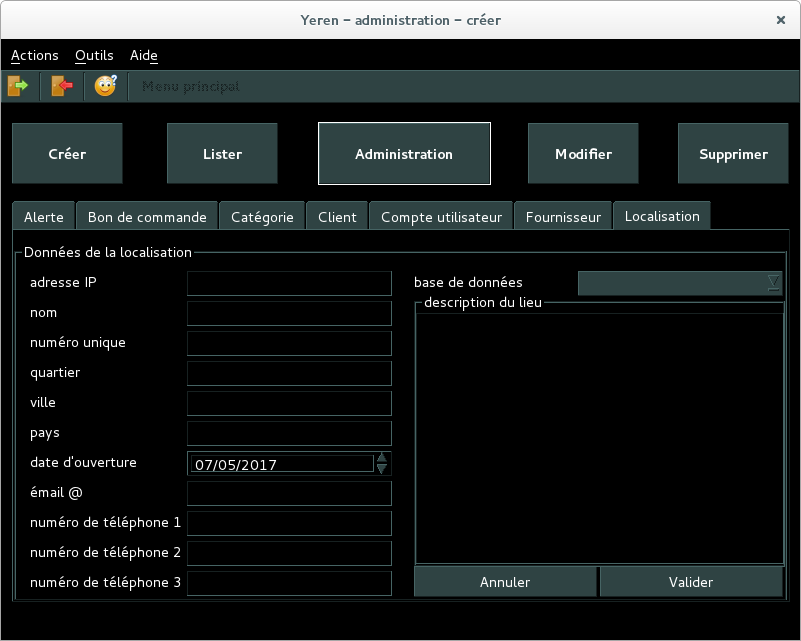
\includegraphics[scale=0.45]{images/localisation-creer.png}
	\caption{L'interface graphique pour cr\'eer une localisation.}
	\label{fig:admin-localisations-creer}
\end{figure}

\procparagraph{Proc\'edure pour cr\'eer une localisation}
\begin{enumerate}[1)]
	\item \`A partir de l'interface graphique de l'acceuil de
		l'administration (voir figure~\ref{fig:fenetre-administrateur}),
		on clique sur l'onglet intitul\'e \textbf{op\'erations}. 
		
	\item Choisir '\textbf{cr\'eer}' dans le '\emph{combo box
		op\'erations}'.
		
	\item Choisir '\textbf{une localisation}' dans
		le '\emph{combo box objets}'. Vous \^etes automatiquement
		conduit \`a la fen\^etre illustr\'ee par la
		figure~\ref{fig:admin-localisations-creer}.
		
	\item Saisissez les informations requises dans les champs
		de texte suivants:
		\begin{enumerate}[1)]
			\item adresse IP 
			\item nom \obligatoire
			\item num\'ero unique 
			\item quartier
			\item ville
			\item province / \'etat
			\item pays
			\item bo\^ite postale
			\item date d'ouverture
			\item \'email@
			\item num\'ero de t\'el\'ephone 1
			\item num\'ero de t\'el\'ephone 2	
			\item base de donn\'ees					
			\item description du lieu.\\
		\end{enumerate}
		
		Si vous avez entr\'e une adresse IP pour cette 
		localisation, vous devez choisir le type de base de
		donn\'ees utilis\'e dans cette localisation. Pour
		l'instant, \yeren ne fonctionne qu'avec \emphbf{MySQL}.\\
		
		La section~\ref{sec:yeren-sgbd} dans
		l'annexe~\ref{chap:environement-logiciel-requis}
		(L'Environnement Logiciel) contient plus d'information
		aux sujets des bases de donn\'ees dans \yeren.
		
	\item Cliquer sur le bouton \bouton{Valider} pour
		valider votre travail.	
\end{enumerate}

%%%%%%%%%%%%%%%%%%%%%%%%%%%%%%%%%%%%%%%%%%%%%%%%%%%%%%%%%%%%%%%%%%%%%%%%%%%%%%%%%

\newpage
\nxsubsection{Lister les localisations}
\index{lister les localisations}

La figure~\ref{fig:admin-localisations-lister} illustre
l'interface graphique de \yeren qui liste les localisations.\\

\begin{figure}[!htpb]
	\centering
	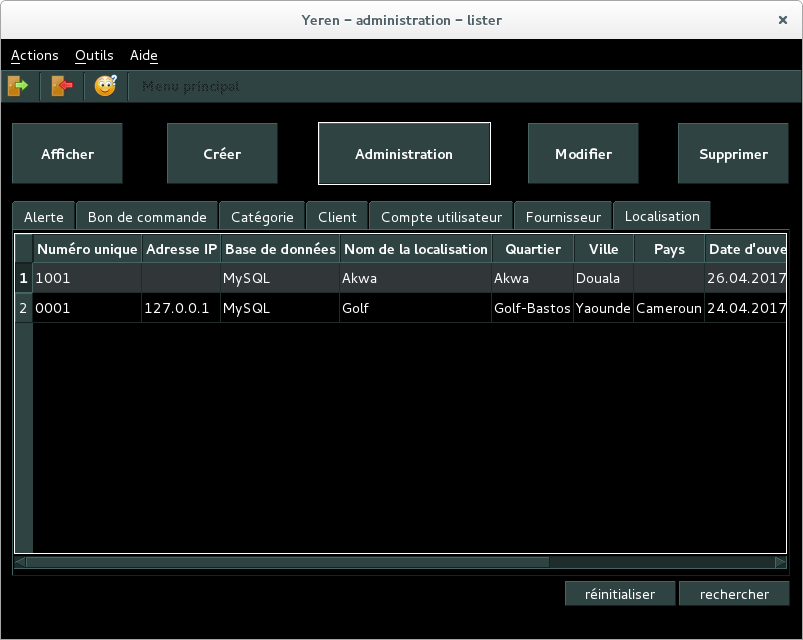
\includegraphics[scale=0.45]{images/localisation-lister.png}
	\caption{L'interface graphique pour cr\'eer une localisation.}
	\label{fig:admin-localisations-lister}
\end{figure}

\procparagraph{Proc\'edure pour lister les localisations}
\begin{enumerate}[1)]
	\item \`A partir de l'interface graphique de l'acceuil de
		l'administration (voir figure~\ref{fig:fenetre-administrateur}),
		on clique sur l'onglet intitul\'e \textbf{op\'erations}. 
		
	\item Choisir '\textbf{lister}' dans le '\emph{combo box
		op\'erations}'.
		
	\item Choisir '\textbf{une localisation}' dans le
		'\emph{combo box objets}'. Vous \^etes automatiquement
		conduit \`a la fen\^etre qui liste localisations
		(figure~\ref{fig:admin-localisations-lister}).
\end{enumerate}

%%%%%%%%%%%%%%%%%%%%%%%%%%%%%%%%%%%%%%%%%%%%%%%%%%%%%%%%%%%%%%%%%%%%%%%%%%%%%%%%%

\newpage
\nxsubsection{Modifier les d\'etails d'une localisation}
\index{modifier les d\'etails d'une localisation}

La figure~\ref{fig:admin-localisations-modifier} illustre
l'interface graphique de \yeren pour modifier les d\'etails
d'une localisation.\\

\begin{figure}[!htpb]
	\centering
	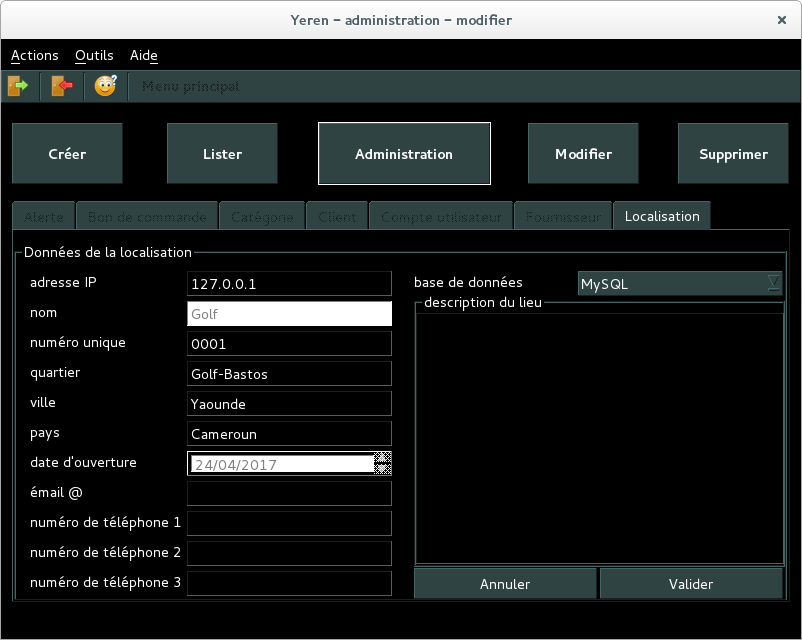
\includegraphics[scale=0.45]{images/localisation-modifier.png}
	\caption{L'interface graphique pour modifier les d\'etails
			d'une localisation.}
	\label{fig:admin-localisations-modifier}
\end{figure}

\procparagraph{Proc\'edure pour modifier les d\'etails d'une localisation}
\begin{enumerate}[1)]
	\item \`A partir de l'interface graphique de l'acceuil de
		l'administration (voir figure~\ref{fig:fenetre-administrateur}),
		on clique sur l'onglet intitul\'e \textbf{op\'erations}. 
		
	\item Choisir '\textbf{lister}' dans le '\emph{combo box
		op\'erations}'.
		
	\item Choisir '\textbf{une localisation}' dans
		le '\emph{combo box objets}'. Vous \^etes automatiquement
		conduit \`a la fen\^etre illustr\'ee par la
		figure~\ref{fig:admin-localisations-lister}.
		
	\item S\'electionner la localisation dont vous souhaitez
		modifier les d\'etails dans la liste des localisations
		affich\'ee.
		
	\item Cliquer sur le bouton \bouton{Modifier}. Les d\'etails
		de la localisation sont affich\'es dans une nouvelle
		fen\^etre.
		
	\item Faites les modifications que vous souhaitez.
		
	\item Cliquer sur le bouton \bouton{valider} pour valider
		les modifications faites.
\end{enumerate}

%%%%%%%%%%%%%%%%%%%%%%%%%%%%%%%%%%%%%%%%%%%%%%%%%%%%%%%%%%%%%%%%%%%%%%%%%%%%%%%%%

%\newpage
\nxsubsection{Supprimer une localisation}
\index{supprimer une localisation}

La figure~\ref{fig:admin-localisations-supprimer} illustre
l'interface graphique de \yeren pour supprimer une localisation.\\

\begin{figure}[!htpb]
	\centering
	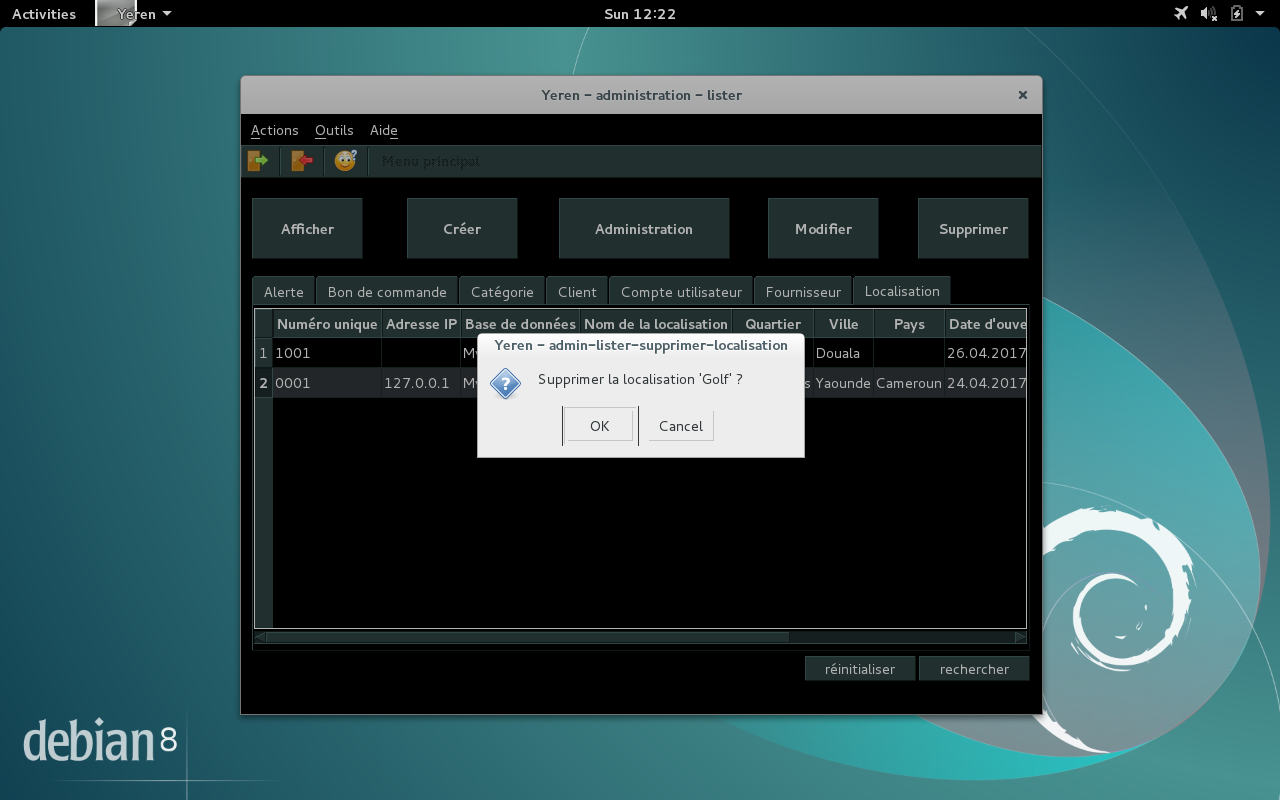
\includegraphics[scale=0.35]{images/localisation-supprimer.png}
	\caption{L'interface graphique pour supprimer une localisation.}
	\label{fig:admin-localisations-supprimer}
\end{figure}

\procparagraph{Proc\'edure pour supprimer une localisation}
\begin{enumerate}[1)]
	\item \`A partir de l'interface graphique de l'acceuil de
		l'administration (voir figure~\ref{fig:fenetre-administrateur}),
		on clique sur l'onglet intitul\'e \textbf{op\'erations}. 
		
	\item Choisir '\textbf{supprimer}' dans le '\emph{combo box
		op\'erations}'.
		
	\item Choisir '\textbf{une localisation}' dans le '\emph{combo box
		sujets}'. Vous \^etes automatiquement conduit \`a la fen\^etre
		illustr\'ee par la figure~\ref{fig:admin-localisations-lister}.
		
	\item S\'electionner la localisation \`a supprimer dans la liste
		des localisations affich\'ee.
		
	\item Cliquer sur le bouton \bouton{Supprimer}. La question
		est ensuite pos\'ee si vous confirmer votre choix.
		Cliquer sur le \bouton{OK} pour confirmer votre choix.
\end{enumerate}


%-----------------------------------------------------------
